\documentclass[twoside]{article}

% Packages required by doxygen
\usepackage{fixltx2e}
\usepackage{calc}
\usepackage{doxygen}
\usepackage{graphicx}
\usepackage[utf8]{inputenc}
\usepackage{makeidx}
\usepackage{multicol}
\usepackage{multirow}
\PassOptionsToPackage{warn}{textcomp}
\usepackage{textcomp}
\usepackage[nointegrals]{wasysym}
\usepackage[table]{xcolor}

% Font selection
\usepackage[T1]{fontenc}
\usepackage{mathptmx}
\usepackage[scaled=.90]{helvet}
\usepackage{courier}
\usepackage{amssymb}
\usepackage{sectsty}
\renewcommand{\familydefault}{\sfdefault}
\allsectionsfont{%
  \fontseries{bc}\selectfont%
  \color{darkgray}%
}
\renewcommand{\DoxyLabelFont}{%
  \fontseries{bc}\selectfont%
  \color{darkgray}%
}
\newcommand{\+}{\discretionary{\mbox{\scriptsize$\hookleftarrow$}}{}{}}

% Page & text layout
\usepackage{geometry}
\geometry{%
  a4paper,%
  top=2.5cm,%
  bottom=2.5cm,%
  left=2.5cm,%
  right=2.5cm%
}
\tolerance=750
\hfuzz=15pt
\hbadness=750
\setlength{\emergencystretch}{15pt}
\setlength{\parindent}{0cm}
\setlength{\parskip}{0.2cm}
\makeatletter
\renewcommand{\paragraph}{%
  \@startsection{paragraph}{4}{0ex}{-1.0ex}{1.0ex}{%
    \normalfont\normalsize\bfseries\SS@parafont%
  }%
}
\renewcommand{\subparagraph}{%
  \@startsection{subparagraph}{5}{0ex}{-1.0ex}{1.0ex}{%
    \normalfont\normalsize\bfseries\SS@subparafont%
  }%
}
\makeatother

% Headers & footers
\usepackage{fancyhdr}
\pagestyle{fancyplain}
\fancyhead[LE]{\fancyplain{}{FEI}}
\fancyhead[CE]{\fancyplain{}{}}
\fancyhead[RE]{\fancyplain{}{KKUI}}
\fancyhead[LO]{\fancyplain{}{FEI}}
\fancyhead[CO]{\fancyplain{}{}}
\fancyhead[RO]{\fancyplain{}{KKUI}}
\fancyfoot[LE]{\fancyplain{}{}}
\fancyfoot[CE]{\fancyplain{}{\bfseries\thepage}}
\fancyfoot[CO]{\fancyplain{}{\bfseries\thepage}}
\fancyfoot[RO]{\fancyplain{}{}}
\renewcommand{\footrulewidth}{0.4pt}
\renewcommand{\sectionmark}[1]{%
  \markright{\thesection\ #1}%
}

% Indices & bibliography
\usepackage{natbib}
\usepackage[titles]{tocloft}
\setcounter{tocdepth}{3}
\setcounter{secnumdepth}{5}
\makeindex

% Hyperlinks (required, but should be loaded last)
\usepackage{ifpdf}
\ifpdf
  \usepackage[pdftex,pagebackref=true]{hyperref}
\else
  \usepackage[ps2pdf,pagebackref=true]{hyperref}
\fi
\hypersetup{%
  colorlinks=true,%
  linkcolor=blue,%
  citecolor=blue,%
  unicode%
}

% Custom commands
\newcommand{\clearemptydoublepage}{%
  \newpage{\pagestyle{empty}\cleardoublepage}%
}


%===== C O N T E N T S =====

\begin{document}

% Titlepage & ToC
\hypersetup{pageanchor=false,
             bookmarks=true,
             bookmarksnumbered=true,
             pdfencoding=unicode
            }
\pagenumbering{roman}
\begin{titlepage}
\end{titlepage}
\tableofcontents
\pagenumbering{arabic}
\hypersetup{pageanchor=true}
%--- Begin generated contents ---
\pagebreak
\vspace*{5em}
\begin{center}%
	\begin{figure}[ht!]
		\centering
		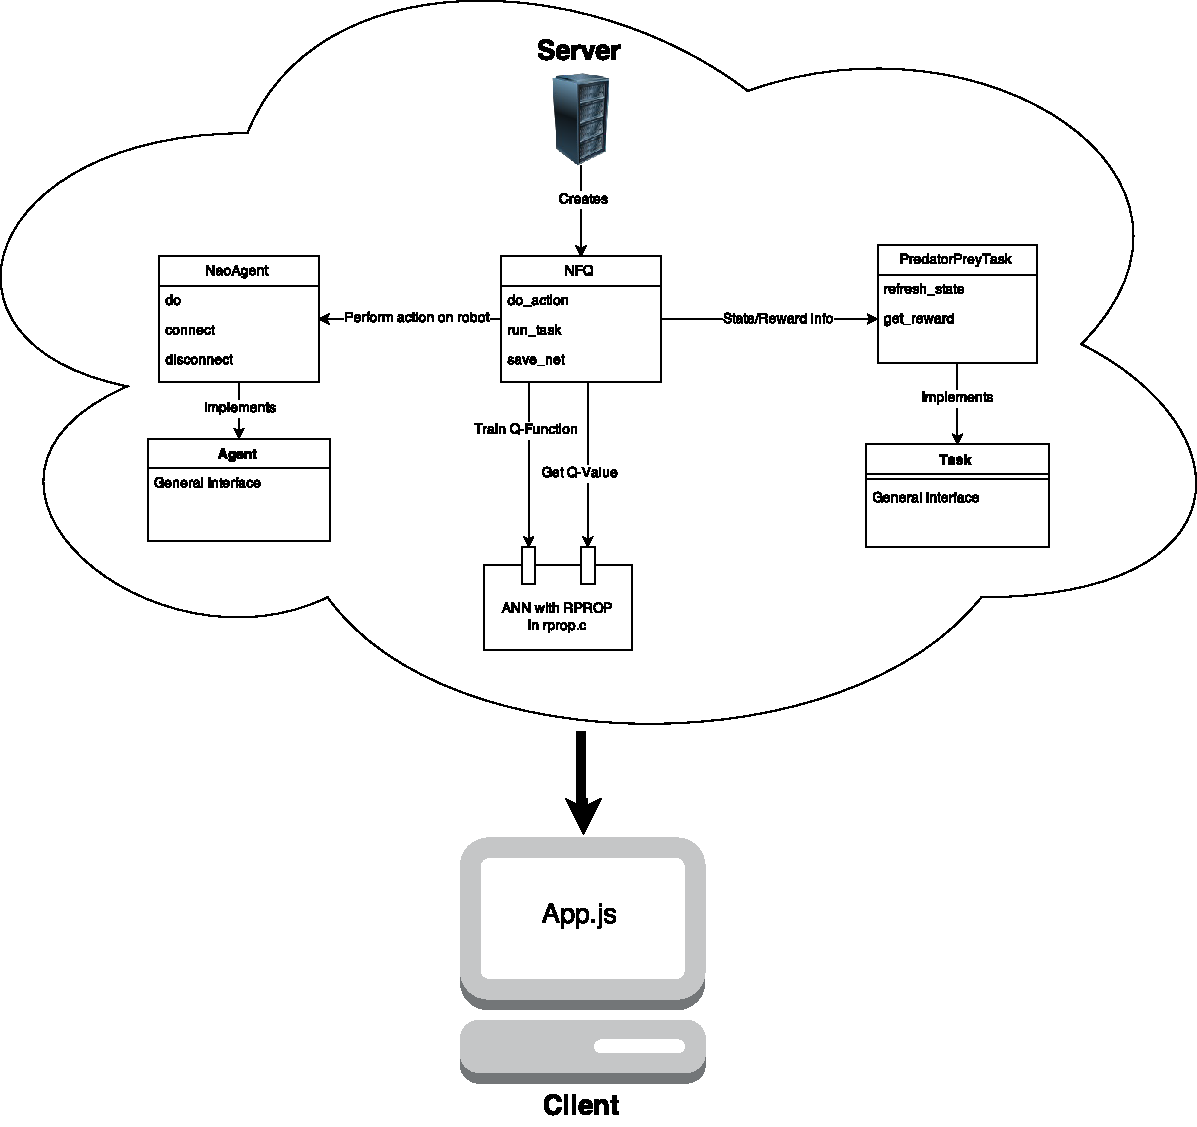
\includegraphics[width=1.0\textwidth]{nfq.pdf}
		\caption{Class/dependency diagram}\label{f:1}
	\end{figure}
\end{center}
\pagebreak
\section{Data Structure Documentation}
\subsection{Agent Class Reference}
\label{class_agent_1_1_agent}\index{Agent@{Agent}}


Provides a default interface for \doxyref{Agent}{p.}{class_agent_1_1_agent} class.  




Inherited by {\bf Nao\+Agent}.

\subsubsection*{Public Member Functions}
\begin{DoxyCompactItemize}
\item 
def {\bf connect}
\begin{DoxyCompactList}\small\item\em This method should handle connection to a real world agent. \end{DoxyCompactList}\item 
def {\bf disconnect}
\begin{DoxyCompactList}\small\item\em This methods should handle disconnection from a real world agent. \end{DoxyCompactList}\item 
def {\bf do}
\begin{DoxyCompactList}\small\item\em This methods handles performing selected action according to action number on a real world agent. \end{DoxyCompactList}\end{DoxyCompactItemize}


\subsubsection{Detailed Description}
Provides a default interface for \doxyref{Agent}{p.}{class_agent_1_1_agent} class. 

\subsubsection{Member Function Documentation}
\index{Agent\+::\+Agent@{Agent\+::\+Agent}!connect@{connect}}
\index{connect@{connect}!Agent\+::\+Agent@{Agent\+::\+Agent}}
\paragraph[{connect}]{\setlength{\rightskip}{0pt plus 5cm}def connect (
\begin{DoxyParamCaption}
\item[{}]{self}
\end{DoxyParamCaption}
)}\label{class_agent_1_1_agent_a0f3e881a92d7a1b4d6d07d9e63180c98}


This method should handle connection to a real world agent. 

This method must be implemented \index{Agent\+::\+Agent@{Agent\+::\+Agent}!disconnect@{disconnect}}
\index{disconnect@{disconnect}!Agent\+::\+Agent@{Agent\+::\+Agent}}
\paragraph[{disconnect}]{\setlength{\rightskip}{0pt plus 5cm}def disconnect (
\begin{DoxyParamCaption}
\item[{}]{self}
\end{DoxyParamCaption}
)}\label{class_agent_1_1_agent_afab97b4023d6e30d95344406b3655983}


This methods should handle disconnection from a real world agent. 

This method must be implemented \index{Agent\+::\+Agent@{Agent\+::\+Agent}!do@{do}}
\index{do@{do}!Agent\+::\+Agent@{Agent\+::\+Agent}}
\paragraph[{do}]{\setlength{\rightskip}{0pt plus 5cm}def do (
\begin{DoxyParamCaption}
\item[{}]{self, }
\item[{}]{action\+\_\+number}
\end{DoxyParamCaption}
)}\label{class_agent_1_1_agent_a412db3f49e4869fa4cb87535dcc77caf}


This methods handles performing selected action according to action number on a real world agent. 

This method must be implemented 
\begin{DoxyParams}{Parameters}
{\em action\+\_\+number} & Number of action to be performed \\
\hline
\end{DoxyParams}


The documentation for this class was generated from the following file\+:\begin{DoxyCompactItemize}
\item 
/home/gomez/\+Projects/\+B\+P/visualization/server/Agent.\+py\end{DoxyCompactItemize}

\subsection{ann\+\_\+t Struct Reference}
\label{structann__t}\index{ann\+\_\+t@{ann\+\_\+t}}


Struct representing a neural network.  


\subsubsection*{Data Fields}
\begin{DoxyCompactItemize}
\item 
double {\bf x} [Nx]
\item 
double {\bf y} [Nx]
\item 
double {\bf delta} [Nx]
\item 
double {\bf prev\+Grad} [Nx][Nx]
\item 
double {\bf curr\+Grad} [Nx][Nx]
\item 
double {\bf update\+Value} [Nx][Nx]
\item 
double {\bf w\+Delta} [Nx][Nx]
\item 
double {\bf w} [Nx][Nx]
\item 
double {\bf dv} [{\bf Nou}]
\end{DoxyCompactItemize}


\subsubsection{Detailed Description}
Struct representing a neural network. 

Container for a complex M\+L\+P structure. 

\subsubsection{Field Documentation}
\index{ann\+\_\+t@{ann\+\_\+t}!curr\+Grad@{curr\+Grad}}
\index{curr\+Grad@{curr\+Grad}!ann\+\_\+t@{ann\+\_\+t}}
\paragraph[{curr\+Grad}]{\setlength{\rightskip}{0pt plus 5cm}double curr\+Grad[Nx][Nx]}\label{structann__t_ad634fb273a77c89ef50752fe62499b4f}
Weight current error gradient \index{ann\+\_\+t@{ann\+\_\+t}!delta@{delta}}
\index{delta@{delta}!ann\+\_\+t@{ann\+\_\+t}}
\paragraph[{delta}]{\setlength{\rightskip}{0pt plus 5cm}double delta[Nx]}\label{structann__t_a610000125df6a3004a1a0768bee350be}
Delta value on neurons \index{ann\+\_\+t@{ann\+\_\+t}!dv@{dv}}
\index{dv@{dv}!ann\+\_\+t@{ann\+\_\+t}}
\paragraph[{dv}]{\setlength{\rightskip}{0pt plus 5cm}double dv[{\bf Nou}]}\label{structann__t_a3cd26d516c0d78e0bd8e83f7b5d96056}
Target value on output neurons \index{ann\+\_\+t@{ann\+\_\+t}!prev\+Grad@{prev\+Grad}}
\index{prev\+Grad@{prev\+Grad}!ann\+\_\+t@{ann\+\_\+t}}
\paragraph[{prev\+Grad}]{\setlength{\rightskip}{0pt plus 5cm}double prev\+Grad[Nx][Nx]}\label{structann__t_ae668825bd99ec5a8e701cd34833d92c8}
Weight error gradient from last step \index{ann\+\_\+t@{ann\+\_\+t}!update\+Value@{update\+Value}}
\index{update\+Value@{update\+Value}!ann\+\_\+t@{ann\+\_\+t}}
\paragraph[{update\+Value}]{\setlength{\rightskip}{0pt plus 5cm}double update\+Value[Nx][Nx]}\label{structann__t_a56f1cf095bad5da7e0c944dd9727293a}
Update value according to R\+P\+R\+O\+P algorithm for each weight \index{ann\+\_\+t@{ann\+\_\+t}!w@{w}}
\index{w@{w}!ann\+\_\+t@{ann\+\_\+t}}
\paragraph[{w}]{\setlength{\rightskip}{0pt plus 5cm}double w[Nx][Nx]}\label{structann__t_aee905c93142ba709a90118c788622185}
Weights matrix \index{ann\+\_\+t@{ann\+\_\+t}!w\+Delta@{w\+Delta}}
\index{w\+Delta@{w\+Delta}!ann\+\_\+t@{ann\+\_\+t}}
\paragraph[{w\+Delta}]{\setlength{\rightskip}{0pt plus 5cm}double w\+Delta[Nx][Nx]}\label{structann__t_a19e899724a3a7ab9150e22e0d48ebc3e}
Delta of weights change \index{ann\+\_\+t@{ann\+\_\+t}!x@{x}}
\index{x@{x}!ann\+\_\+t@{ann\+\_\+t}}
\paragraph[{x}]{\setlength{\rightskip}{0pt plus 5cm}double x[Nx]}\label{structann__t_ac566dbcdd25e058c1e82f59d63dfd12b}
Input of neurons \index{ann\+\_\+t@{ann\+\_\+t}!y@{y}}
\index{y@{y}!ann\+\_\+t@{ann\+\_\+t}}
\paragraph[{y}]{\setlength{\rightskip}{0pt plus 5cm}double y[Nx]}\label{structann__t_adec9cbbd838a286742a4ae286bff0e30}
Output of neurons 

The documentation for this struct was generated from the following file\+:\begin{DoxyCompactItemize}
\item 
/home/gomez/\+Projects/\+B\+P/visualization/server/{\bf rprop.\+c}\end{DoxyCompactItemize}

\subsection{Main\+Handler Class Reference}
\label{classserver_1_1_main_handler}\index{Main\+Handler@{Main\+Handler}}


Operates a web server for web application.  




Inherits Request\+Handler.

\subsubsection*{Public Member Functions}
\begin{DoxyCompactItemize}
\item 
def {\bf get}
\begin{DoxyCompactList}\small\item\em Handles asynchronous web request and renders a web app. \end{DoxyCompactList}\end{DoxyCompactItemize}


\subsubsection{Detailed Description}
Operates a web server for web application. 

\subsubsection{Member Function Documentation}
\index{server\+::\+Main\+Handler@{server\+::\+Main\+Handler}!get@{get}}
\index{get@{get}!server\+::\+Main\+Handler@{server\+::\+Main\+Handler}}
\paragraph[{get}]{\setlength{\rightskip}{0pt plus 5cm}def get (
\begin{DoxyParamCaption}
\item[{}]{request}
\end{DoxyParamCaption}
)}\label{classserver_1_1_main_handler_a444a1328efb32d5d9d2dcb2efe855d3b}


Handles asynchronous web request and renders a web app. 


\begin{DoxyParams}{Parameters}
{\em request} & Web request received \\
\hline
\end{DoxyParams}


The documentation for this class was generated from the following file\+:\begin{DoxyCompactItemize}
\item 
/home/gomez/\+Projects/\+B\+P/visualization/server/server.\+py\end{DoxyCompactItemize}

\subsection{Nao\+Agent Class Reference}
\label{class_nao_agent_1_1_nao_agent}\index{Nao\+Agent@{Nao\+Agent}}


Implementation of Agent interface on Nao robot in Webots simulator.  




Inherits {\bf Agent}.

\subsubsection*{Public Member Functions}
\begin{DoxyCompactItemize}
\item 
def {\bf \+\_\+\+\_\+init\+\_\+\+\_\+}\label{class_nao_agent_1_1_nao_agent_ac775ee34451fdfa742b318538164070e}

\begin{DoxyCompactList}\small\item\em Constructor method setups default parameters. \end{DoxyCompactList}\item 
def {\bf connect}
\begin{DoxyCompactList}\small\item\em Method handles connection to simulated robot and initialization of its features. \end{DoxyCompactList}\item 
def {\bf disconnect}\label{class_nao_agent_1_1_nao_agent_afab97b4023d6e30d95344406b3655983}

\begin{DoxyCompactList}\small\item\em Disconnects from simulated Nao. \end{DoxyCompactList}\item 
def {\bf do}
\begin{DoxyCompactList}\small\item\em Perform specified action from the set of all available motions. \end{DoxyCompactList}\item 
def {\bf go\+\_\+forward}\label{class_nao_agent_1_1_nao_agent_a74f88e9c727035ad050d4a1b5e16eb5f}

\begin{DoxyCompactList}\small\item\em This method performs movements along the X-\/axis, with 0.\+25m distance. \end{DoxyCompactList}\item 
def {\bf go\+\_\+right}\label{class_nao_agent_1_1_nao_agent_a1825cf4236b693f347db9c793206049c}

\begin{DoxyCompactList}\small\item\em This method performs a rotation 30 degrees to the right. \end{DoxyCompactList}\item 
def {\bf go\+\_\+left}\label{class_nao_agent_1_1_nao_agent_a3661eec663302a3b67351833c2c9b8de}

\begin{DoxyCompactList}\small\item\em This method perform movement 30 degrees left. \end{DoxyCompactList}\item 
def {\bf Stiffness\+On}
\begin{DoxyCompactList}\small\item\em Sets the stiffnes of Nao's joints to maximal value, to make him ready to perform motions. \end{DoxyCompactList}\end{DoxyCompactItemize}
\subsubsection*{Data Fields}
\begin{DoxyCompactItemize}
\item 
{\bf robot\+\_\+ip}\label{class_nao_agent_1_1_nao_agent_a70221305bf8db6392330ef28121efd25}

\begin{DoxyCompactList}\small\item\em Default connection I\+P address. \end{DoxyCompactList}\item 
{\bf robot\+\_\+port}\label{class_nao_agent_1_1_nao_agent_a9282cdfa59976fe1cfc1a539df185c27}

\begin{DoxyCompactList}\small\item\em Default connection port. \end{DoxyCompactList}\end{DoxyCompactItemize}


\subsubsection{Detailed Description}
Implementation of Agent interface on Nao robot in Webots simulator. 

\subsubsection{Member Function Documentation}
\index{Nao\+Agent\+::\+Nao\+Agent@{Nao\+Agent\+::\+Nao\+Agent}!connect@{connect}}
\index{connect@{connect}!Nao\+Agent\+::\+Nao\+Agent@{Nao\+Agent\+::\+Nao\+Agent}}
\paragraph[{connect}]{\setlength{\rightskip}{0pt plus 5cm}def connect (
\begin{DoxyParamCaption}
\item[{}]{self, }
\item[{}]{ip = {\ttfamily None}, }
\item[{}]{port = {\ttfamily None}}
\end{DoxyParamCaption}
)}\label{class_nao_agent_1_1_nao_agent_a0f3e881a92d7a1b4d6d07d9e63180c98}


Method handles connection to simulated robot and initialization of its features. 

It connection to the robot on specified Ip\+:port and initializes the robot to the init position, preparing it for motions. 
\begin{DoxyParams}{Parameters}
{\em ip} & I\+P address of a robot \\
\hline
{\em port} & Port number of a robot \\
\hline
\end{DoxyParams}
\begin{DoxyReturn}{Returns}
True, if connection was succesful, else False 
\end{DoxyReturn}
\index{Nao\+Agent\+::\+Nao\+Agent@{Nao\+Agent\+::\+Nao\+Agent}!do@{do}}
\index{do@{do}!Nao\+Agent\+::\+Nao\+Agent@{Nao\+Agent\+::\+Nao\+Agent}}
\paragraph[{do}]{\setlength{\rightskip}{0pt plus 5cm}def do (
\begin{DoxyParamCaption}
\item[{}]{self, }
\item[{}]{action\+\_\+number}
\end{DoxyParamCaption}
)}\label{class_nao_agent_1_1_nao_agent_a412db3f49e4869fa4cb87535dcc77caf}


Perform specified action from the set of all available motions. 


\begin{DoxyParams}{Parameters}
{\em action\+\_\+number} & specifies position of action in the action list \\
\hline
\end{DoxyParams}
\index{Nao\+Agent\+::\+Nao\+Agent@{Nao\+Agent\+::\+Nao\+Agent}!Stiffness\+On@{Stiffness\+On}}
\index{Stiffness\+On@{Stiffness\+On}!Nao\+Agent\+::\+Nao\+Agent@{Nao\+Agent\+::\+Nao\+Agent}}
\paragraph[{Stiffness\+On}]{\setlength{\rightskip}{0pt plus 5cm}def Stiffness\+On (
\begin{DoxyParamCaption}
\item[{}]{self, }
\item[{}]{proxy}
\end{DoxyParamCaption}
)}\label{class_nao_agent_1_1_nao_agent_add7585e99624d7863d2e1291b1af2669}


Sets the stiffnes of Nao's joints to maximal value, to make him ready to perform motions. 


\begin{DoxyParams}{Parameters}
{\em proxy} & specifies a proxy(path) for setting the joint's stiffness \\
\hline
\end{DoxyParams}


The documentation for this class was generated from the following file\+:\begin{DoxyCompactItemize}
\item 
/home/gomez/\+Projects/\+B\+P/visualization/server/Nao\+Agent.\+py\end{DoxyCompactItemize}

\hypertarget{class_n_f_q_1_1_n_f_q}{\subsection{N\+F\+Q Class Reference}
\label{class_n_f_q_1_1_n_f_q}\index{N\+F\+Q@{N\+F\+Q}}
}


This class handles mechanism behind \hyperlink{class_n_f_q_1_1_n_f_q}{N\+F\+Q} learning and also decision process.  


\subsubsection*{Public Member Functions}
\begin{DoxyCompactItemize}
\item 
def \hyperlink{class_n_f_q_1_1_n_f_q_ac775ee34451fdfa742b318538164070e}{\+\_\+\+\_\+init\+\_\+\+\_\+}
\begin{DoxyCompactList}\small\item\em Constructor of the class. \end{DoxyCompactList}\item 
def \hyperlink{class_n_f_q_1_1_n_f_q_a6b708400f5bc84a9084858995ec0e1e3}{save\+\_\+net}
\begin{DoxyCompactList}\small\item\em Saves current network to database. \end{DoxyCompactList}\item 
def \hyperlink{class_n_f_q_1_1_n_f_q_ace29d26dedd78bf2aa11a7a6a4963ba1}{load\+\_\+net}
\begin{DoxyCompactList}\small\item\em Loads and update current network weights with the network saved in database. \end{DoxyCompactList}\item 
def \hyperlink{class_n_f_q_1_1_n_f_q_af8c46da13010e428234320546345b43b}{load\+\_\+tasks}
\begin{DoxyCompactList}\small\item\em Loads a list of all previously learned tasks from a database. \end{DoxyCompactList}\item 
\hypertarget{class_n_f_q_1_1_n_f_q_a825de7cd4b9446c695dc6f7d53a486e9}{def \hyperlink{class_n_f_q_1_1_n_f_q_a825de7cd4b9446c695dc6f7d53a486e9}{load\+\_\+samples}}\label{class_n_f_q_1_1_n_f_q_a825de7cd4b9446c695dc6f7d53a486e9}

\begin{DoxyCompactList}\small\item\em Loads a previously collected samples from the database and update current ones with them. \end{DoxyCompactList}\item 
\hypertarget{class_n_f_q_1_1_n_f_q_a049ce9e8a989730486b24d334489a6b6}{def \hyperlink{class_n_f_q_1_1_n_f_q_a049ce9e8a989730486b24d334489a6b6}{write\+\_\+samples}}\label{class_n_f_q_1_1_n_f_q_a049ce9e8a989730486b24d334489a6b6}

\begin{DoxyCompactList}\small\item\em Upload current training samples set into database in J\+S\+O\+N format. \end{DoxyCompactList}\item 
def \hyperlink{class_n_f_q_1_1_n_f_q_aed1f496109cb75fd667748796f70af1a}{sample\+\_\+to\+\_\+patterns}
\begin{DoxyCompactList}\small\item\em This method provides basic transformation from the training sample into training patterns. \end{DoxyCompactList}\item 
def \hyperlink{class_n_f_q_1_1_n_f_q_a41bb19974711e6fdc955751d5c1c0fa0}{get\+\_\+training\+\_\+set\+\_\+from\+\_\+samples}
\begin{DoxyCompactList}\small\item\em Transform whole set of training samples into training patterns according to the proposed algorithm. \end{DoxyCompactList}\item 
def \hyperlink{class_n_f_q_1_1_n_f_q_aeb9339921d4a63f47fd93e7d7822f0e1}{learn}
\begin{DoxyCompactList}\small\item\em The key method of this class, if target state is reached, this method updates a current Q-\/function. \end{DoxyCompactList}\item 
def \hyperlink{class_n_f_q_1_1_n_f_q_a334280030ebb62b511dc4849136cee46}{choose\+\_\+controller}
\begin{DoxyCompactList}\small\item\em This method controls the decision process according to current autonomy level. \end{DoxyCompactList}\item 
def \hyperlink{class_n_f_q_1_1_n_f_q_a0647f518d9a29328eed53c958fd3bec9}{run\+\_\+task}
\begin{DoxyCompactList}\small\item\em Runs a task saved in database with a specific name. \end{DoxyCompactList}\item 
def \hyperlink{class_n_f_q_1_1_n_f_q_aada248b40fdbcbd978b62a0deb9f3aff}{make\+\_\+step\+\_\+task}
\begin{DoxyCompactList}\small\item\em This methods handles steps and reward counting during performing loaded tasks. \end{DoxyCompactList}\item 
def \hyperlink{class_n_f_q_1_1_n_f_q_a059828e7afb0a89671ef08f9f9e8c12e}{do\+\_\+action}
\begin{DoxyCompactList}\small\item\em Method representing an elementary step of agent in the environment. \end{DoxyCompactList}\item 
def \hyperlink{class_n_f_q_1_1_n_f_q_aecbff2e71eacc518b89558411e9c4e2a}{get\+Q}
\begin{DoxyCompactList}\small\item\em General method for acquiring the Q-\/value for current state-\/action pair. \end{DoxyCompactList}\item 
def \hyperlink{class_n_f_q_1_1_n_f_q_a3bb0ca0e6444e78d72f843ea687fec56}{min\+Q}
\begin{DoxyCompactList}\small\item\em Gets a minimum Q-\/value in current state for available actions. \end{DoxyCompactList}\item 
def \hyperlink{class_n_f_q_1_1_n_f_q_a5eb62d0f60ade3959535d6c96d9de3c6}{min\+Q\+\_\+index}
\begin{DoxyCompactList}\small\item\em Gets an index of action with minimal Q-\/value in current state. \end{DoxyCompactList}\item 
def \hyperlink{class_n_f_q_1_1_n_f_q_a594aeec3e63750a0d60dc75c883e5412}{max\+Q}
\begin{DoxyCompactList}\small\item\em Gets a maximal Q-\/value in current state for available actions. \end{DoxyCompactList}\item 
def \hyperlink{class_n_f_q_1_1_n_f_q_a73a9b088ceb7051798debf8fa69b148f}{max\+Q\+\_\+index}
\begin{DoxyCompactList}\small\item\em Gets an index of action with a maximal Q-\/value in current state. \end{DoxyCompactList}\item 
def \hyperlink{class_n_f_q_1_1_n_f_q_a009c94bdd435c7a379adda4f47ba7da0}{get\+\_\+target}
\begin{DoxyCompactList}\small\item\em Calculates a target Q-\/value according to Bellman equation mentioned in the work. \end{DoxyCompactList}\end{DoxyCompactItemize}
\subsubsection*{Data Fields}
\begin{DoxyCompactItemize}
\item 
\hypertarget{class_n_f_q_1_1_n_f_q_ab127f2768fff9c4628c413617137a553}{\hyperlink{class_n_f_q_1_1_n_f_q_ab127f2768fff9c4628c413617137a553}{agent}}\label{class_n_f_q_1_1_n_f_q_ab127f2768fff9c4628c413617137a553}

\begin{DoxyCompactList}\small\item\em An Agent performs actions in the environment. \end{DoxyCompactList}\item 
\hypertarget{class_n_f_q_1_1_n_f_q_aa4d42044193f96ecc0d82daab68fb0e6}{\hyperlink{class_n_f_q_1_1_n_f_q_aa4d42044193f96ecc0d82daab68fb0e6}{task}}\label{class_n_f_q_1_1_n_f_q_aa4d42044193f96ecc0d82daab68fb0e6}

\begin{DoxyCompactList}\small\item\em A Task object provides reward function and also environment state update. \end{DoxyCompactList}\item 
\hypertarget{class_n_f_q_1_1_n_f_q_a0d28f70b9b7238e7de23f1128d858d39}{\hyperlink{class_n_f_q_1_1_n_f_q_a0d28f70b9b7238e7de23f1128d858d39}{connected}}\label{class_n_f_q_1_1_n_f_q_a0d28f70b9b7238e7de23f1128d858d39}

\begin{DoxyCompactList}\small\item\em State variable signalizing if Agent is connected to the real robot. \end{DoxyCompactList}\item 
\hypertarget{class_n_f_q_1_1_n_f_q_abf5ffecefbeb3e5456add44dfd66adea}{\hyperlink{class_n_f_q_1_1_n_f_q_abf5ffecefbeb3e5456add44dfd66adea}{redis\+\_\+server}}\label{class_n_f_q_1_1_n_f_q_abf5ffecefbeb3e5456add44dfd66adea}

\begin{DoxyCompactList}\small\item\em Connection to the Redis database. \end{DoxyCompactList}\item 
\hypertarget{class_n_f_q_1_1_n_f_q_a2a24c3eb11c4493c51536a7125927b65}{\hyperlink{class_n_f_q_1_1_n_f_q_a2a24c3eb11c4493c51536a7125927b65}{epoch}}\label{class_n_f_q_1_1_n_f_q_a2a24c3eb11c4493c51536a7125927b65}

\begin{DoxyCompactList}\small\item\em Episode counter. \end{DoxyCompactList}\item 
\hypertarget{class_n_f_q_1_1_n_f_q_a97746837457f12b6a4277c3d459a1b1d}{\hyperlink{class_n_f_q_1_1_n_f_q_a97746837457f12b6a4277c3d459a1b1d}{discount}}\label{class_n_f_q_1_1_n_f_q_a97746837457f12b6a4277c3d459a1b1d}

\begin{DoxyCompactList}\small\item\em Discount factor constant for learning process. \end{DoxyCompactList}\item 
\hypertarget{class_n_f_q_1_1_n_f_q_a6b288a470bcb2fd5f321915ef4045b8b}{\hyperlink{class_n_f_q_1_1_n_f_q_a6b288a470bcb2fd5f321915ef4045b8b}{network}}\label{class_n_f_q_1_1_n_f_q_a6b288a470bcb2fd5f321915ef4045b8b}

\begin{DoxyCompactList}\small\item\em Holds weights of the neural network. \end{DoxyCompactList}\item 
\hypertarget{class_n_f_q_1_1_n_f_q_a95accbf9778b78efc6b4605f4d909eb8}{\hyperlink{class_n_f_q_1_1_n_f_q_a95accbf9778b78efc6b4605f4d909eb8}{samples}}\label{class_n_f_q_1_1_n_f_q_a95accbf9778b78efc6b4605f4d909eb8}

\begin{DoxyCompactList}\small\item\em Set of training samples in a form of tuples according to work. \end{DoxyCompactList}\item 
\hypertarget{class_n_f_q_1_1_n_f_q_ab87fb1dc8a9c886db84a2fa17729eaf9}{\hyperlink{class_n_f_q_1_1_n_f_q_ab87fb1dc8a9c886db84a2fa17729eaf9}{training\+\_\+set}}\label{class_n_f_q_1_1_n_f_q_ab87fb1dc8a9c886db84a2fa17729eaf9}

\begin{DoxyCompactList}\small\item\em Set of training pattern, which can be applied directly to the neural network. \end{DoxyCompactList}\item 
\hypertarget{class_n_f_q_1_1_n_f_q_adc6e5733fc3c22f0a7b2914188c49c90}{\hyperlink{class_n_f_q_1_1_n_f_q_adc6e5733fc3c22f0a7b2914188c49c90}{state}}\label{class_n_f_q_1_1_n_f_q_adc6e5733fc3c22f0a7b2914188c49c90}

\begin{DoxyCompactList}\small\item\em Representation of environment state. \end{DoxyCompactList}\item 
\hypertarget{class_n_f_q_1_1_n_f_q_aaa8f1acc9fab510954fe555060a241b2}{\hyperlink{class_n_f_q_1_1_n_f_q_aaa8f1acc9fab510954fe555060a241b2}{step\+\_\+counter}}\label{class_n_f_q_1_1_n_f_q_aaa8f1acc9fab510954fe555060a241b2}

\begin{DoxyCompactList}\small\item\em Counts steps made during current episode. \end{DoxyCompactList}\end{DoxyCompactItemize}
\subsubsection*{Static Public Attributes}
\begin{DoxyCompactItemize}
\item 
\hypertarget{class_n_f_q_1_1_n_f_q_a9cec28f2b80d53fea0778e72264a1b2a}{list \hyperlink{class_n_f_q_1_1_n_f_q_a9cec28f2b80d53fea0778e72264a1b2a}{action\+\_\+codes}}\label{class_n_f_q_1_1_n_f_q_a9cec28f2b80d53fea0778e72264a1b2a}

\begin{DoxyCompactList}\small\item\em Encoding of action number for purposes of neural network input. \end{DoxyCompactList}\end{DoxyCompactItemize}


\subsubsection{Detailed Description}
This class handles mechanism behind \hyperlink{class_n_f_q_1_1_n_f_q}{N\+F\+Q} learning and also decision process. 

It contains definitions for methods that handles communication with database, operating the neural network, performing tasks and finally the \hyperlink{class_n_f_q_1_1_n_f_q}{N\+F\+Q} learning and decision procedure. \begin{DoxyVerb}@author Jan Gamec
@version 1.0
\end{DoxyVerb}
 

\subsubsection{Constructor \& Destructor Documentation}
\hypertarget{class_n_f_q_1_1_n_f_q_ac775ee34451fdfa742b318538164070e}{\index{N\+F\+Q\+::\+N\+F\+Q@{N\+F\+Q\+::\+N\+F\+Q}!\+\_\+\+\_\+init\+\_\+\+\_\+@{\+\_\+\+\_\+init\+\_\+\+\_\+}}
\index{\+\_\+\+\_\+init\+\_\+\+\_\+@{\+\_\+\+\_\+init\+\_\+\+\_\+}!N\+F\+Q\+::\+N\+F\+Q@{N\+F\+Q\+::\+N\+F\+Q}}
\paragraph[{\+\_\+\+\_\+init\+\_\+\+\_\+}]{\setlength{\rightskip}{0pt plus 5cm}def \+\_\+\+\_\+init\+\_\+\+\_\+ (
\begin{DoxyParamCaption}
\item[{}]{self, }
\item[{}]{discount = {\ttfamily 0.99}}
\end{DoxyParamCaption}
)}}\label{class_n_f_q_1_1_n_f_q_ac775ee34451fdfa742b318538164070e}


Constructor of the class. 

Handles basic configuration of the \hyperlink{class_n_f_q_1_1_n_f_q}{N\+F\+Q} module and its constants. It's arranging connection with Redis database and initializes Agent and Task objects, that are necessary for algorithm. It handles initialization of neural network keeping learned knowledge if no record of network configuration is in database. It also loads information about previous learning process from the database and parses previous samples intro training patterns. 
\begin{DoxyParams}{Parameters}
{\em discount} & Discount factor constant used during learning \\
\hline
\end{DoxyParams}


\subsubsection{Member Function Documentation}
\hypertarget{class_n_f_q_1_1_n_f_q_a334280030ebb62b511dc4849136cee46}{\index{N\+F\+Q\+::\+N\+F\+Q@{N\+F\+Q\+::\+N\+F\+Q}!choose\+\_\+controller@{choose\+\_\+controller}}
\index{choose\+\_\+controller@{choose\+\_\+controller}!N\+F\+Q\+::\+N\+F\+Q@{N\+F\+Q\+::\+N\+F\+Q}}
\paragraph[{choose\+\_\+controller}]{\setlength{\rightskip}{0pt plus 5cm}def choose\+\_\+controller (
\begin{DoxyParamCaption}
\item[{}]{self}
\end{DoxyParamCaption}
)}}\label{class_n_f_q_1_1_n_f_q_a334280030ebb62b511dc4849136cee46}


This method controls the decision process according to current autonomy level. 

It either asks a humna operator for action or decides according to the policy \hypertarget{class_n_f_q_1_1_n_f_q_a059828e7afb0a89671ef08f9f9e8c12e}{\index{N\+F\+Q\+::\+N\+F\+Q@{N\+F\+Q\+::\+N\+F\+Q}!do\+\_\+action@{do\+\_\+action}}
\index{do\+\_\+action@{do\+\_\+action}!N\+F\+Q\+::\+N\+F\+Q@{N\+F\+Q\+::\+N\+F\+Q}}
\paragraph[{do\+\_\+action}]{\setlength{\rightskip}{0pt plus 5cm}def do\+\_\+action (
\begin{DoxyParamCaption}
\item[{}]{self, }
\item[{}]{action\+\_\+num, }
\item[{}]{autonomy = {\ttfamily False}}
\end{DoxyParamCaption}
)}}\label{class_n_f_q_1_1_n_f_q_a059828e7afb0a89671ef08f9f9e8c12e}


Method representing an elementary step of agent in the environment. 

Given the action number, method make an Agent do selected action and collect a sample information. Samples are collected in a tuples according to work. \begin{quote}
\mbox{[}state at t, action number, state at t+1, epoch, step\mbox{]} \end{quote}
If total autonomy (in a case of performing leaded task) is off, sample is appended to current sample set. This method then delegates decision process back to the \hyperlink{class_n_f_q_1_1_n_f_q_aeb9339921d4a63f47fd93e7d7822f0e1}{learn()} method in a recursive way 
\begin{DoxyParams}{Parameters}
{\em action\+\_\+num} & Number of action in the action set \\
\hline
{\em autonomy} & Default value is False. During autonomy samples are not stored \\
\hline
\end{DoxyParams}
\hypertarget{class_n_f_q_1_1_n_f_q_a009c94bdd435c7a379adda4f47ba7da0}{\index{N\+F\+Q\+::\+N\+F\+Q@{N\+F\+Q\+::\+N\+F\+Q}!get\+\_\+target@{get\+\_\+target}}
\index{get\+\_\+target@{get\+\_\+target}!N\+F\+Q\+::\+N\+F\+Q@{N\+F\+Q\+::\+N\+F\+Q}}
\paragraph[{get\+\_\+target}]{\setlength{\rightskip}{0pt plus 5cm}def get\+\_\+target (
\begin{DoxyParamCaption}
\item[{}]{self, }
\item[{}]{state = {\ttfamily None}, }
\item[{}]{step = {\ttfamily None}}
\end{DoxyParamCaption}
)}}\label{class_n_f_q_1_1_n_f_q_a009c94bdd435c7a379adda4f47ba7da0}


Calculates a target Q-\/value according to Bellman equation mentioned in the work. 


\begin{DoxyParams}{Parameters}
{\em state} & Represents an environment state. Default is current state. \\
\hline
{\em step} & Time step. Default value is step count in current episode \\
\hline
\end{DoxyParams}
\begin{DoxyReturn}{Returns}
Returns the target Q-\/value for a neural network training 
\end{DoxyReturn}
\hypertarget{class_n_f_q_1_1_n_f_q_a41bb19974711e6fdc955751d5c1c0fa0}{\index{N\+F\+Q\+::\+N\+F\+Q@{N\+F\+Q\+::\+N\+F\+Q}!get\+\_\+training\+\_\+set\+\_\+from\+\_\+samples@{get\+\_\+training\+\_\+set\+\_\+from\+\_\+samples}}
\index{get\+\_\+training\+\_\+set\+\_\+from\+\_\+samples@{get\+\_\+training\+\_\+set\+\_\+from\+\_\+samples}!N\+F\+Q\+::\+N\+F\+Q@{N\+F\+Q\+::\+N\+F\+Q}}
\paragraph[{get\+\_\+training\+\_\+set\+\_\+from\+\_\+samples}]{\setlength{\rightskip}{0pt plus 5cm}def get\+\_\+training\+\_\+set\+\_\+from\+\_\+samples (
\begin{DoxyParamCaption}
\item[{}]{self}
\end{DoxyParamCaption}
)}}\label{class_n_f_q_1_1_n_f_q_a41bb19974711e6fdc955751d5c1c0fa0}


Transform whole set of training samples into training patterns according to the proposed algorithm. 

This method updates current training set used for training with the generated one \hypertarget{class_n_f_q_1_1_n_f_q_aecbff2e71eacc518b89558411e9c4e2a}{\index{N\+F\+Q\+::\+N\+F\+Q@{N\+F\+Q\+::\+N\+F\+Q}!get\+Q@{get\+Q}}
\index{get\+Q@{get\+Q}!N\+F\+Q\+::\+N\+F\+Q@{N\+F\+Q\+::\+N\+F\+Q}}
\paragraph[{get\+Q}]{\setlength{\rightskip}{0pt plus 5cm}def get\+Q (
\begin{DoxyParamCaption}
\item[{}]{self, }
\item[{}]{state, }
\item[{}]{operator}
\end{DoxyParamCaption}
)}}\label{class_n_f_q_1_1_n_f_q_aecbff2e71eacc518b89558411e9c4e2a}


General method for acquiring the Q-\/value for current state-\/action pair. 

This method runs a neural network forward in order to get Q-\/value for current state 
\begin{DoxyParams}{Parameters}
{\em state} & Represents state of environment \\
\hline
{\em operator} & Function handle, e.\+g. we want minimal Q-\/value in current state for available actions, we use function min() \\
\hline
\end{DoxyParams}
\begin{DoxyReturn}{Returns}
A pair, where first value corresponds to the actual Q-\/value and second is the index of the action having this value 
\end{DoxyReturn}
\hypertarget{class_n_f_q_1_1_n_f_q_aeb9339921d4a63f47fd93e7d7822f0e1}{\index{N\+F\+Q\+::\+N\+F\+Q@{N\+F\+Q\+::\+N\+F\+Q}!learn@{learn}}
\index{learn@{learn}!N\+F\+Q\+::\+N\+F\+Q@{N\+F\+Q\+::\+N\+F\+Q}}
\paragraph[{learn}]{\setlength{\rightskip}{0pt plus 5cm}def learn (
\begin{DoxyParamCaption}
\item[{}]{self}
\end{DoxyParamCaption}
)}}\label{class_n_f_q_1_1_n_f_q_aeb9339921d4a63f47fd93e7d7822f0e1}


The key method of this class, if target state is reached, this method updates a current Q-\/function. 

Update is realised training a neural network with a training patternset generated from samples collected during previous episodes. It also updates information about the learning progress to the database (Episode no., Number of steps) It delegates recursive control process to the \hyperlink{class_n_f_q_1_1_n_f_q_a334280030ebb62b511dc4849136cee46}{choose\+\_\+controller} \begin{DoxySeeAlso}{See also}
\hyperlink{class_n_f_q_1_1_n_f_q_a334280030ebb62b511dc4849136cee46}{choose\+\_\+controller} method 
\end{DoxySeeAlso}
\hypertarget{class_n_f_q_1_1_n_f_q_ace29d26dedd78bf2aa11a7a6a4963ba1}{\index{N\+F\+Q\+::\+N\+F\+Q@{N\+F\+Q\+::\+N\+F\+Q}!load\+\_\+net@{load\+\_\+net}}
\index{load\+\_\+net@{load\+\_\+net}!N\+F\+Q\+::\+N\+F\+Q@{N\+F\+Q\+::\+N\+F\+Q}}
\paragraph[{load\+\_\+net}]{\setlength{\rightskip}{0pt plus 5cm}def load\+\_\+net (
\begin{DoxyParamCaption}
\item[{}]{self, }
\item[{}]{name = {\ttfamily 'net'}}
\end{DoxyParamCaption}
)}}\label{class_n_f_q_1_1_n_f_q_ace29d26dedd78bf2aa11a7a6a4963ba1}


Loads and update current network weights with the network saved in database. 


\begin{DoxyParams}{Parameters}
{\em name} & Specifies the name of network in the database \\
\hline
\end{DoxyParams}
\hypertarget{class_n_f_q_1_1_n_f_q_af8c46da13010e428234320546345b43b}{\index{N\+F\+Q\+::\+N\+F\+Q@{N\+F\+Q\+::\+N\+F\+Q}!load\+\_\+tasks@{load\+\_\+tasks}}
\index{load\+\_\+tasks@{load\+\_\+tasks}!N\+F\+Q\+::\+N\+F\+Q@{N\+F\+Q\+::\+N\+F\+Q}}
\paragraph[{load\+\_\+tasks}]{\setlength{\rightskip}{0pt plus 5cm}def load\+\_\+tasks (
\begin{DoxyParamCaption}
\item[{}]{self}
\end{DoxyParamCaption}
)}}\label{class_n_f_q_1_1_n_f_q_af8c46da13010e428234320546345b43b}


Loads a list of all previously learned tasks from a database. 

\begin{DoxyReturn}{Returns}
List of all learned tasks 
\end{DoxyReturn}
\hypertarget{class_n_f_q_1_1_n_f_q_aada248b40fdbcbd978b62a0deb9f3aff}{\index{N\+F\+Q\+::\+N\+F\+Q@{N\+F\+Q\+::\+N\+F\+Q}!make\+\_\+step\+\_\+task@{make\+\_\+step\+\_\+task}}
\index{make\+\_\+step\+\_\+task@{make\+\_\+step\+\_\+task}!N\+F\+Q\+::\+N\+F\+Q@{N\+F\+Q\+::\+N\+F\+Q}}
\paragraph[{make\+\_\+step\+\_\+task}]{\setlength{\rightskip}{0pt plus 5cm}def make\+\_\+step\+\_\+task (
\begin{DoxyParamCaption}
\item[{}]{self, }
\item[{}]{reward = {\ttfamily 0}}
\end{DoxyParamCaption}
)}}\label{class_n_f_q_1_1_n_f_q_aada248b40fdbcbd978b62a0deb9f3aff}


This methods handles steps and reward counting during performing loaded tasks. 

It works in the recursive way. If target area or step limit is not reached, agent make a step and cumulate the reward. The method calls itself until target state or step limit is reached. 
\begin{DoxyParams}{Parameters}
{\em reward} & Represents current cumulative reward \\
\hline
\end{DoxyParams}
\begin{DoxyReturn}{Returns}
Reward after end of task performance 
\end{DoxyReturn}
\hypertarget{class_n_f_q_1_1_n_f_q_a594aeec3e63750a0d60dc75c883e5412}{\index{N\+F\+Q\+::\+N\+F\+Q@{N\+F\+Q\+::\+N\+F\+Q}!max\+Q@{max\+Q}}
\index{max\+Q@{max\+Q}!N\+F\+Q\+::\+N\+F\+Q@{N\+F\+Q\+::\+N\+F\+Q}}
\paragraph[{max\+Q}]{\setlength{\rightskip}{0pt plus 5cm}def max\+Q (
\begin{DoxyParamCaption}
\item[{}]{self, }
\item[{}]{state}
\end{DoxyParamCaption}
)}}\label{class_n_f_q_1_1_n_f_q_a594aeec3e63750a0d60dc75c883e5412}


Gets a maximal Q-\/value in current state for available actions. 


\begin{DoxyParams}{Parameters}
{\em state} & Represents state of environment \\
\hline
\end{DoxyParams}
\begin{DoxyReturn}{Returns}
maximal Q-\/value for current state 
\end{DoxyReturn}
\hypertarget{class_n_f_q_1_1_n_f_q_a73a9b088ceb7051798debf8fa69b148f}{\index{N\+F\+Q\+::\+N\+F\+Q@{N\+F\+Q\+::\+N\+F\+Q}!max\+Q\+\_\+index@{max\+Q\+\_\+index}}
\index{max\+Q\+\_\+index@{max\+Q\+\_\+index}!N\+F\+Q\+::\+N\+F\+Q@{N\+F\+Q\+::\+N\+F\+Q}}
\paragraph[{max\+Q\+\_\+index}]{\setlength{\rightskip}{0pt plus 5cm}def max\+Q\+\_\+index (
\begin{DoxyParamCaption}
\item[{}]{self, }
\item[{}]{state}
\end{DoxyParamCaption}
)}}\label{class_n_f_q_1_1_n_f_q_a73a9b088ceb7051798debf8fa69b148f}


Gets an index of action with a maximal Q-\/value in current state. 


\begin{DoxyParams}{Parameters}
{\em state} & Represents state of environment \\
\hline
\end{DoxyParams}
\begin{DoxyReturn}{Returns}
Index of the action with a maximal Q-\/value 
\end{DoxyReturn}
\hypertarget{class_n_f_q_1_1_n_f_q_a3bb0ca0e6444e78d72f843ea687fec56}{\index{N\+F\+Q\+::\+N\+F\+Q@{N\+F\+Q\+::\+N\+F\+Q}!min\+Q@{min\+Q}}
\index{min\+Q@{min\+Q}!N\+F\+Q\+::\+N\+F\+Q@{N\+F\+Q\+::\+N\+F\+Q}}
\paragraph[{min\+Q}]{\setlength{\rightskip}{0pt plus 5cm}def min\+Q (
\begin{DoxyParamCaption}
\item[{}]{self, }
\item[{}]{state}
\end{DoxyParamCaption}
)}}\label{class_n_f_q_1_1_n_f_q_a3bb0ca0e6444e78d72f843ea687fec56}


Gets a minimum Q-\/value in current state for available actions. 


\begin{DoxyParams}{Parameters}
{\em state} & Represents state of environment \\
\hline
\end{DoxyParams}
\begin{DoxyReturn}{Returns}
Minimal Q-\/value for current state 
\end{DoxyReturn}
\hypertarget{class_n_f_q_1_1_n_f_q_a5eb62d0f60ade3959535d6c96d9de3c6}{\index{N\+F\+Q\+::\+N\+F\+Q@{N\+F\+Q\+::\+N\+F\+Q}!min\+Q\+\_\+index@{min\+Q\+\_\+index}}
\index{min\+Q\+\_\+index@{min\+Q\+\_\+index}!N\+F\+Q\+::\+N\+F\+Q@{N\+F\+Q\+::\+N\+F\+Q}}
\paragraph[{min\+Q\+\_\+index}]{\setlength{\rightskip}{0pt plus 5cm}def min\+Q\+\_\+index (
\begin{DoxyParamCaption}
\item[{}]{self, }
\item[{}]{state}
\end{DoxyParamCaption}
)}}\label{class_n_f_q_1_1_n_f_q_a5eb62d0f60ade3959535d6c96d9de3c6}


Gets an index of action with minimal Q-\/value in current state. 


\begin{DoxyParams}{Parameters}
{\em state} & Represents state of environment \\
\hline
\end{DoxyParams}
\begin{DoxyReturn}{Returns}
Index of the action with minimal Q-\/value 
\end{DoxyReturn}
\hypertarget{class_n_f_q_1_1_n_f_q_a0647f518d9a29328eed53c958fd3bec9}{\index{N\+F\+Q\+::\+N\+F\+Q@{N\+F\+Q\+::\+N\+F\+Q}!run\+\_\+task@{run\+\_\+task}}
\index{run\+\_\+task@{run\+\_\+task}!N\+F\+Q\+::\+N\+F\+Q@{N\+F\+Q\+::\+N\+F\+Q}}
\paragraph[{run\+\_\+task}]{\setlength{\rightskip}{0pt plus 5cm}def run\+\_\+task (
\begin{DoxyParamCaption}
\item[{}]{self, }
\item[{}]{name}
\end{DoxyParamCaption}
)}}\label{class_n_f_q_1_1_n_f_q_a0647f518d9a29328eed53c958fd3bec9}


Runs a task saved in database with a specific name. 

The learned task is represented by its N\+N weights configuration which are loaded and replaces current network configuration during the task performance. Original network is restored after then. 
\begin{DoxyParams}{Parameters}
{\em name} & Specifies a name of task saved in database \\
\hline
\end{DoxyParams}
\begin{DoxyReturn}{Returns}
Returns cumulative reward after task was performed 
\end{DoxyReturn}
\hypertarget{class_n_f_q_1_1_n_f_q_aed1f496109cb75fd667748796f70af1a}{\index{N\+F\+Q\+::\+N\+F\+Q@{N\+F\+Q\+::\+N\+F\+Q}!sample\+\_\+to\+\_\+patterns@{sample\+\_\+to\+\_\+patterns}}
\index{sample\+\_\+to\+\_\+patterns@{sample\+\_\+to\+\_\+patterns}!N\+F\+Q\+::\+N\+F\+Q@{N\+F\+Q\+::\+N\+F\+Q}}
\paragraph[{sample\+\_\+to\+\_\+patterns}]{\setlength{\rightskip}{0pt plus 5cm}def sample\+\_\+to\+\_\+patterns (
\begin{DoxyParamCaption}
\item[{}]{self, }
\item[{}]{sample}
\end{DoxyParamCaption}
)}}\label{class_n_f_q_1_1_n_f_q_aed1f496109cb75fd667748796f70af1a}


This method provides basic transformation from the training sample into training patterns. 

Training patterns are generated according to the algorithm in the work, where for action selected in sample pattern with minimal Q-\/value is generated and for all other actions patterns with maximal Q are generated 
\begin{DoxyParams}{Parameters}
{\em sample} & Training sample in the form of tuple \\
\hline
\end{DoxyParams}
\begin{DoxyReturn}{Returns}
List of training patterns 
\end{DoxyReturn}
\hypertarget{class_n_f_q_1_1_n_f_q_a6b708400f5bc84a9084858995ec0e1e3}{\index{N\+F\+Q\+::\+N\+F\+Q@{N\+F\+Q\+::\+N\+F\+Q}!save\+\_\+net@{save\+\_\+net}}
\index{save\+\_\+net@{save\+\_\+net}!N\+F\+Q\+::\+N\+F\+Q@{N\+F\+Q\+::\+N\+F\+Q}}
\paragraph[{save\+\_\+net}]{\setlength{\rightskip}{0pt plus 5cm}def save\+\_\+net (
\begin{DoxyParamCaption}
\item[{}]{self, }
\item[{}]{name = {\ttfamily 'net'}}
\end{DoxyParamCaption}
)}}\label{class_n_f_q_1_1_n_f_q_a6b708400f5bc84a9084858995ec0e1e3}


Saves current network to database. 


\begin{DoxyParams}{Parameters}
{\em name} & Specifies name for the network \\
\hline
\end{DoxyParams}


The documentation for this class was generated from the following file\+:\begin{DoxyCompactItemize}
\item 
N\+F\+Q.\+py\end{DoxyCompactItemize}

\subsection{Predator\+Prey\+Task Class Reference}
\label{class_predator_prey_task_1_1_predator_prey_task}\index{Predator\+Prey\+Task@{Predator\+Prey\+Task}}


Implementation of Task interface for a so called Predator-\/\+Prey task.  




Inherits {\bf Task}.

\subsubsection*{Public Member Functions}
\begin{DoxyCompactItemize}
\item 
def {\bf \+\_\+\+\_\+init\+\_\+\+\_\+}\label{class_predator_prey_task_1_1_predator_prey_task_ac775ee34451fdfa742b318538164070e}

\begin{DoxyCompactList}\small\item\em Constructor method. \end{DoxyCompactList}\item 
def {\bf get\+\_\+reward}
\begin{DoxyCompactList}\small\item\em A reward function. \end{DoxyCompactList}\item 
def {\bf refresh\+\_\+state}
\begin{DoxyCompactList}\small\item\em Update current state loading the data from database. \end{DoxyCompactList}\end{DoxyCompactItemize}
\subsubsection*{Data Fields}
\begin{DoxyCompactItemize}
\item 
{\bf database}\label{class_predator_prey_task_1_1_predator_prey_task_a64dbaa3229ec575b68ec333442e10cee}

\begin{DoxyCompactList}\small\item\em Handles connection to the Redis database. \end{DoxyCompactList}\item 
{\bf state}\label{class_predator_prey_task_1_1_predator_prey_task_adc6e5733fc3c22f0a7b2914188c49c90}

\begin{DoxyCompactList}\small\item\em Stores current state. \end{DoxyCompactList}\end{DoxyCompactItemize}


\subsubsection{Detailed Description}
Implementation of Task interface for a so called Predator-\/\+Prey task. 

\subsubsection{Member Function Documentation}
\index{Predator\+Prey\+Task\+::\+Predator\+Prey\+Task@{Predator\+Prey\+Task\+::\+Predator\+Prey\+Task}!get\+\_\+reward@{get\+\_\+reward}}
\index{get\+\_\+reward@{get\+\_\+reward}!Predator\+Prey\+Task\+::\+Predator\+Prey\+Task@{Predator\+Prey\+Task\+::\+Predator\+Prey\+Task}}
\paragraph[{get\+\_\+reward}]{\setlength{\rightskip}{0pt plus 5cm}def get\+\_\+reward (
\begin{DoxyParamCaption}
\item[{}]{self, }
\item[{}]{state}
\end{DoxyParamCaption}
)}\label{class_predator_prey_task_1_1_predator_prey_task_aa97b81cdb2e9a08c63eab0ca7e94bf66}


A reward function. 

If agent is closer to target than 0.\+5m cca 0.\+15 normalized and rotated less than 30 degrees, its considered to be a target state so the reward is 0. Else reward is equal 0.\+01 
\begin{DoxyParams}{Parameters}
{\em state} & Current environment state \\
\hline
\end{DoxyParams}
\begin{DoxyReturn}{Returns}
Returns a reward for a give state 
\end{DoxyReturn}
\index{Predator\+Prey\+Task\+::\+Predator\+Prey\+Task@{Predator\+Prey\+Task\+::\+Predator\+Prey\+Task}!refresh\+\_\+state@{refresh\+\_\+state}}
\index{refresh\+\_\+state@{refresh\+\_\+state}!Predator\+Prey\+Task\+::\+Predator\+Prey\+Task@{Predator\+Prey\+Task\+::\+Predator\+Prey\+Task}}
\paragraph[{refresh\+\_\+state}]{\setlength{\rightskip}{0pt plus 5cm}def refresh\+\_\+state (
\begin{DoxyParamCaption}
\item[{}]{self}
\end{DoxyParamCaption}
)}\label{class_predator_prey_task_1_1_predator_prey_task_a09e7b7d13235130045548d33b3352a1d}


Update current state loading the data from database. 

\begin{DoxyReturn}{Returns}
Returns current environment state 
\end{DoxyReturn}


The documentation for this class was generated from the following file\+:\begin{DoxyCompactItemize}
\item 
/home/gomez/\+Projects/\+B\+P/visualization/server/Predator\+Prey\+Task.\+py\end{DoxyCompactItemize}

\subsection{Task Class Reference}
\label{class_task_1_1_task}\index{Task@{Task}}


Provides a default interface for Tasks used in N\+F\+Q.  




Inherited by {\bf Predator\+Prey\+Task}.

\subsubsection*{Public Member Functions}
\begin{DoxyCompactItemize}
\item 
def {\bf get\+\_\+reward}
\begin{DoxyCompactList}\small\item\em Reward function. \end{DoxyCompactList}\item 
def {\bf refresh\+\_\+state}
\begin{DoxyCompactList}\small\item\em Method for updating environment state. \end{DoxyCompactList}\end{DoxyCompactItemize}


\subsubsection{Detailed Description}
Provides a default interface for Tasks used in N\+F\+Q. 

\subsubsection{Member Function Documentation}
\index{Task\+::\+Task@{Task\+::\+Task}!get\+\_\+reward@{get\+\_\+reward}}
\index{get\+\_\+reward@{get\+\_\+reward}!Task\+::\+Task@{Task\+::\+Task}}
\paragraph[{get\+\_\+reward}]{\setlength{\rightskip}{0pt plus 5cm}def get\+\_\+reward (
\begin{DoxyParamCaption}
\item[{}]{self, }
\item[{}]{state}
\end{DoxyParamCaption}
)}\label{class_task_1_1_task_aa97b81cdb2e9a08c63eab0ca7e94bf66}


Reward function. 

This method has to be implemented \index{Task\+::\+Task@{Task\+::\+Task}!refresh\+\_\+state@{refresh\+\_\+state}}
\index{refresh\+\_\+state@{refresh\+\_\+state}!Task\+::\+Task@{Task\+::\+Task}}
\paragraph[{refresh\+\_\+state}]{\setlength{\rightskip}{0pt plus 5cm}def refresh\+\_\+state (
\begin{DoxyParamCaption}
\item[{}]{self}
\end{DoxyParamCaption}
)}\label{class_task_1_1_task_a09e7b7d13235130045548d33b3352a1d}


Method for updating environment state. 

This method has to be implemented 

The documentation for this class was generated from the following file\+:\begin{DoxyCompactItemize}
\item 
/home/gomez/\+Projects/\+B\+P/visualization/server/Task.\+py\end{DoxyCompactItemize}

\hypertarget{classserver_1_1_w_s_handler}{\subsection{W\+S\+Handler Class Reference}
\label{classserver_1_1_w_s_handler}\index{W\+S\+Handler@{W\+S\+Handler}}
}


Handles websocket communication with web app.  




Inherits Web\+Socket\+Handler.

\subsubsection*{Public Member Functions}
\begin{DoxyCompactItemize}
\item 
def \hyperlink{classserver_1_1_w_s_handler_ae4b82667a73596ae2d8042e9b4be8a95}{open}
\begin{DoxyCompactList}\small\item\em Handles all new connections. \end{DoxyCompactList}\item 
def \hyperlink{classserver_1_1_w_s_handler_a7618f0d180e9433d4fda68fdcc77b883}{on\+\_\+message}
\begin{DoxyCompactList}\small\item\em Handles various type of messages received over W\+S. \end{DoxyCompactList}\item 
\hypertarget{classserver_1_1_w_s_handler_a278f5ae83d49aaff3f84e571d3af6f47}{def \hyperlink{classserver_1_1_w_s_handler_a278f5ae83d49aaff3f84e571d3af6f47}{on\+\_\+close}}\label{classserver_1_1_w_s_handler_a278f5ae83d49aaff3f84e571d3af6f47}

\begin{DoxyCompactList}\small\item\em Handles close of W\+S connection from client. \end{DoxyCompactList}\end{DoxyCompactItemize}


\subsubsection{Detailed Description}
Handles websocket communication with web app. 

\subsubsection{Member Function Documentation}
\hypertarget{classserver_1_1_w_s_handler_a7618f0d180e9433d4fda68fdcc77b883}{\index{server\+::\+W\+S\+Handler@{server\+::\+W\+S\+Handler}!on\+\_\+message@{on\+\_\+message}}
\index{on\+\_\+message@{on\+\_\+message}!server\+::\+W\+S\+Handler@{server\+::\+W\+S\+Handler}}
\paragraph[{on\+\_\+message}]{\setlength{\rightskip}{0pt plus 5cm}def on\+\_\+message (
\begin{DoxyParamCaption}
\item[{}]{self, }
\item[{}]{json\+\_\+message}
\end{DoxyParamCaption}
)}}\label{classserver_1_1_w_s_handler_a7618f0d180e9433d4fda68fdcc77b883}


Handles various type of messages received over W\+S. 

It distinc 3 main commands\+:
\begin{DoxyItemize}
\item Performing an action.
\item Saving current task.
\item Running loaded task.
\end{DoxyItemize}

It also responds with corresponding data 
\begin{DoxyParams}{Parameters}
{\em json\+\_\+message} & Data received in W\+S request (like action number) \\
\hline
\end{DoxyParams}
\hypertarget{classserver_1_1_w_s_handler_ae4b82667a73596ae2d8042e9b4be8a95}{\index{server\+::\+W\+S\+Handler@{server\+::\+W\+S\+Handler}!open@{open}}
\index{open@{open}!server\+::\+W\+S\+Handler@{server\+::\+W\+S\+Handler}}
\paragraph[{open}]{\setlength{\rightskip}{0pt plus 5cm}def open (
\begin{DoxyParamCaption}
\item[{}]{self}
\end{DoxyParamCaption}
)}}\label{classserver_1_1_w_s_handler_ae4b82667a73596ae2d8042e9b4be8a95}


Handles all new connections. 

Initializes a new N\+F\+Q instance for each new W\+S connection 

The documentation for this class was generated from the following file\+:\begin{DoxyCompactItemize}
\item 
server.\+py\end{DoxyCompactItemize}

\section{File Documentation}
\section{\+\_\+rprop.\+c File Reference}
\label{__rprop_8c}\index{\+\_\+rprop.\+c@{\+\_\+rprop.\+c}}


File containing python wrapper for a C M\+L\+P with R\+P\+R\+O\+P.  


{\ttfamily \#include $<$Python.\+h$>$}\\*
{\ttfamily \#include $<$numpy/arrayobject.\+h$>$}\\*
{\ttfamily \#include \char`\"{}rprop.\+c\char`\"{}}\\*
\subsection*{Functions}
\begin{DoxyCompactItemize}
\item 
static Py\+Object $\ast$ {\bf rprop\+\_\+learn2} (Py\+Object $\ast$self, Py\+Object $\ast$args)
\begin{DoxyCompactList}\small\item\em Function wrapping a learning process of a neural network. \end{DoxyCompactList}\item 
static Py\+Object $\ast$ {\bf rprop\+\_\+run2} (Py\+Object $\ast$self, Py\+Object $\ast$args)
\begin{DoxyCompactList}\small\item\em Function wrapping a function that runs a neural network forward. \end{DoxyCompactList}\item 
static Py\+Object $\ast$ {\bf rprop\+\_\+init} (Py\+Object $\ast$self, Py\+Object $\ast$args)
\begin{DoxyCompactList}\small\item\em Function wrapping a initialization of a network. \end{DoxyCompactList}\item 
Py\+M\+O\+D\+I\+N\+I\+T\+\_\+\+F\+U\+N\+C {\bf init\+\_\+rprop} (void)\label{__rprop_8c_af5e1e1f1114b87ddbcf2a656ebaae392}

\begin{DoxyCompactList}\small\item\em Initializes python wrapping functions. \end{DoxyCompactList}\end{DoxyCompactItemize}
\subsection*{Variables}
\begin{DoxyCompactItemize}
\item 
static Py\+Method\+Def {\bf module\+\_\+methods} [$\,$]
\end{DoxyCompactItemize}


\subsection{Detailed Description}
File containing python wrapper for a C M\+L\+P with R\+P\+R\+O\+P. 

\begin{DoxyAuthor}{Author}
Jan Gamec 
\end{DoxyAuthor}
\begin{DoxyDate}{Date}
24 May 2015 This file serves as a wrapper for functionality in \doxyref{rprop.\+c}{p.}{rprop_8c} . After building this script, it can be imported as a standalone python module. The module can be build by following command\+: python setup.\+py build\+\_\+ext --inplace
\end{DoxyDate}
The setup.\+py file {\bfseries is required} to be in the same directory as this script!. In order to change configuration of network, please see documentation for \doxyref{rprop.\+c}{p.}{rprop_8c} file. \begin{DoxySeeAlso}{See also}
\doxyref{rprop.\+c}{p.}{rprop_8c} 
\end{DoxySeeAlso}


\subsection{Function Documentation}
\index{\+\_\+rprop.\+c@{\+\_\+rprop.\+c}!rprop\+\_\+init@{rprop\+\_\+init}}
\index{rprop\+\_\+init@{rprop\+\_\+init}!\+\_\+rprop.\+c@{\+\_\+rprop.\+c}}
\subsubsection[{rprop\+\_\+init}]{\setlength{\rightskip}{0pt plus 5cm}static Py\+Object $\ast$ rprop\+\_\+init (
\begin{DoxyParamCaption}
\item[{Py\+Object $\ast$}]{self, }
\item[{Py\+Object $\ast$}]{args}
\end{DoxyParamCaption}
)\hspace{0.3cm}{\ttfamily [static]}}\label{__rprop_8c_a05ecab9c1ec8658b749c787e0c7eb624}


Function wrapping a initialization of a network. 

Function in python has no input arguments. It just creates new network with random weights initialization and return this weights as a numpy array. 
\begin{DoxyParams}{Parameters}
{\em self} & Object pointer \\
\hline
{\em args} & Holds all arguments that can be passed to function in python \\
\hline
\end{DoxyParams}
\begin{DoxyReturn}{Returns}
A numpy array holding new weights of the created network 
\end{DoxyReturn}
\index{\+\_\+rprop.\+c@{\+\_\+rprop.\+c}!rprop\+\_\+learn2@{rprop\+\_\+learn2}}
\index{rprop\+\_\+learn2@{rprop\+\_\+learn2}!\+\_\+rprop.\+c@{\+\_\+rprop.\+c}}
\subsubsection[{rprop\+\_\+learn2}]{\setlength{\rightskip}{0pt plus 5cm}static Py\+Object $\ast$ rprop\+\_\+learn2 (
\begin{DoxyParamCaption}
\item[{Py\+Object $\ast$}]{self, }
\item[{Py\+Object $\ast$}]{args}
\end{DoxyParamCaption}
)\hspace{0.3cm}{\ttfamily [static]}}\label{__rprop_8c_ac719ec79037d0deae73b9dbc1d19c50c}


Function wrapping a learning process of a neural network. 

Function in python accepts following arguments\+:
\begin{DoxyItemize}
\item {\bfseries num\+\_\+of\+\_\+epochs} Number of training epochs
\item {\bfseries pattern\+Set} A numpy array of training patterns
\item {\bfseries weights} A numpy array of neural network weights 
\begin{DoxyParams}{Parameters}
{\em self} & Object pointer \\
\hline
{\em args} & Holds all arguments that can be passed to function in python \\
\hline
\end{DoxyParams}
\begin{DoxyReturn}{Returns}
A numpy array holding new weights 
\end{DoxyReturn}

\end{DoxyItemize}\index{\+\_\+rprop.\+c@{\+\_\+rprop.\+c}!rprop\+\_\+run2@{rprop\+\_\+run2}}
\index{rprop\+\_\+run2@{rprop\+\_\+run2}!\+\_\+rprop.\+c@{\+\_\+rprop.\+c}}
\subsubsection[{rprop\+\_\+run2}]{\setlength{\rightskip}{0pt plus 5cm}static Py\+Object $\ast$ rprop\+\_\+run2 (
\begin{DoxyParamCaption}
\item[{Py\+Object $\ast$}]{self, }
\item[{Py\+Object $\ast$}]{args}
\end{DoxyParamCaption}
)\hspace{0.3cm}{\ttfamily [static]}}\label{__rprop_8c_a0400d0ba1e3b32d144afd89dbf726153}


Function wrapping a function that runs a neural network forward. 

It runs network forward and return values on output neurons. Function in python accepts following arguments\+:
\begin{DoxyItemize}
\item {\bfseries pattern} A numpy array representing one input pattern
\item {\bfseries weights} A numpy array of neural network weights 
\begin{DoxyParams}{Parameters}
{\em self} & Object pointer \\
\hline
{\em args} & Holds all arguments that can be passed to function in python \\
\hline
\end{DoxyParams}
\begin{DoxyReturn}{Returns}
An Q-\/value on the output neuron with double precission 
\end{DoxyReturn}

\end{DoxyItemize}

\subsection{Variable Documentation}
\index{\+\_\+rprop.\+c@{\+\_\+rprop.\+c}!module\+\_\+methods@{module\+\_\+methods}}
\index{module\+\_\+methods@{module\+\_\+methods}!\+\_\+rprop.\+c@{\+\_\+rprop.\+c}}
\subsubsection[{module\+\_\+methods}]{\setlength{\rightskip}{0pt plus 5cm}Py\+Method\+Def module\+\_\+methods[$\,$]\hspace{0.3cm}{\ttfamily [static]}}\label{__rprop_8c_afcd2b5e08091d3973eb552badcfec160}
{\bfseries Initial value\+:}
\begin{DoxyCode}
= \{
  \{\textcolor{stringliteral}{"learn"}, rprop_learn2, METH\_VARARGS, learn\_docstring\},
  \{\textcolor{stringliteral}{"run"}, rprop_run2, METH\_VARARGS, run\_docstring\},
  \{\textcolor{stringliteral}{"init"}, rprop_init, METH\_VARARGS, init\_docstring\},
  \{NULL, NULL, 0, NULL\}
\}
\end{DoxyCode}
Definition of all functions available after the build. 
\hypertarget{app_8js}{\subsection{app.\+js File Reference}
\label{app_8js}\index{app.\+js@{app.\+js}}
}


Javascript application for visualisation of N\+F\+Q algorithm.  


\subsubsection*{Functions}
\begin{DoxyCompactItemize}
\item 
function \hyperlink{app_8js_ae99733c6a0b9e6b556349d5b8b13bc9b}{connect\+Robot} ()
\begin{DoxyCompactList}\small\item\em Initializes new websocket connection to server. \end{DoxyCompactList}\item 
function \hyperlink{app_8js_ace9e4b8a0d6d7e7a149f3af777bb2cb2}{server\+Response} (response)
\begin{DoxyCompactList}\small\item\em Parses received message object from websocket connection. \end{DoxyCompactList}\item 
function \hyperlink{app_8js_a278287ec616d0559012a30c6722d79eb}{show\+Intro} (msg)
\begin{DoxyCompactList}\small\item\em Displays a introduction page. \end{DoxyCompactList}\item 
function \hyperlink{app_8js_a33590eb3c0abc20d4dd4ad2f7b5c88d5}{show\+Controls} ()
\begin{DoxyCompactList}\small\item\em Displays a N\+F\+Q controls and state information. \end{DoxyCompactList}\item 
function \hyperlink{app_8js_a56d8af57b035e728a6862cc68e871a54}{save\+Task} ()
\begin{DoxyCompactList}\small\item\em Request saving current task progress to the database. \end{DoxyCompactList}\item 
function \hyperlink{app_8js_a1cf166da37e318ccdc62ee859a7459c1}{load\+Tasks} (tasks)
\begin{DoxyCompactList}\small\item\em Creates a table of all available tasks from D\+B. \end{DoxyCompactList}\item 
function \hyperlink{app_8js_a1848bc621f7d2a17ff27dee023b1e52b}{run\+Task} (task)
\begin{DoxyCompactList}\small\item\em Requests a server to perform a task on a robot. \end{DoxyCompactList}\item 
function \hyperlink{app_8js_a592b15e55d202ab09969e5f9dc146103}{do\+Action} (action\+\_\+num)
\begin{DoxyCompactList}\small\item\em Order a robot to do selected action. \end{DoxyCompactList}\item 
function \hyperlink{app_8js_afe89789aeb53da0bac57df6583fb9322}{enable\+All\+Buttons} ()
\begin{DoxyCompactList}\small\item\em Enables all buttons on page. \end{DoxyCompactList}\item 
function \hyperlink{app_8js_ab27044ede2517ab019a7d91d08e64e78}{disable\+All\+Buttons} ()
\begin{DoxyCompactList}\small\item\em Disables all buttons on the page to block request until the current action is finished. \end{DoxyCompactList}\item 
function \hyperlink{app_8js_a57727d5a6134f7b88b2d09dfa6667f26}{update\+State} (distance, angle)
\begin{DoxyCompactList}\small\item\em Updates current state information with a new, received over Websocket. \end{DoxyCompactList}\end{DoxyCompactItemize}


\subsubsection{Detailed Description}
Javascript application for visualisation of N\+F\+Q algorithm. 

\begin{DoxyAuthor}{Author}
Jan Gamec 
\end{DoxyAuthor}
\begin{DoxyDate}{Date}
24 May 2015
\end{DoxyDate}
This application is served as a webpage when running the server application. 

\subsubsection{Function Documentation}
\hypertarget{app_8js_ae99733c6a0b9e6b556349d5b8b13bc9b}{\index{app.\+js@{app.\+js}!connect\+Robot@{connect\+Robot}}
\index{connect\+Robot@{connect\+Robot}!app.\+js@{app.\+js}}
\paragraph[{connect\+Robot}]{\setlength{\rightskip}{0pt plus 5cm}function connect\+Robot (
\begin{DoxyParamCaption}
{}
\end{DoxyParamCaption}
)}}\label{app_8js_ae99733c6a0b9e6b556349d5b8b13bc9b}


Initializes new websocket connection to server. 

Establishes a connection to robot through opening a new websocket connection to server. In addition it binds corresponding callbacks for websocket events. When a new message is received, function server\+Response is called, with a received object. \hypertarget{app_8js_ab27044ede2517ab019a7d91d08e64e78}{\index{app.\+js@{app.\+js}!disable\+All\+Buttons@{disable\+All\+Buttons}}
\index{disable\+All\+Buttons@{disable\+All\+Buttons}!app.\+js@{app.\+js}}
\paragraph[{disable\+All\+Buttons}]{\setlength{\rightskip}{0pt plus 5cm}function disable\+All\+Buttons (
\begin{DoxyParamCaption}
{}
\end{DoxyParamCaption}
)}}\label{app_8js_ab27044ede2517ab019a7d91d08e64e78}


Disables all buttons on the page to block request until the current action is finished. 

\hypertarget{app_8js_a592b15e55d202ab09969e5f9dc146103}{\index{app.\+js@{app.\+js}!do\+Action@{do\+Action}}
\index{do\+Action@{do\+Action}!app.\+js@{app.\+js}}
\paragraph[{do\+Action}]{\setlength{\rightskip}{0pt plus 5cm}function do\+Action (
\begin{DoxyParamCaption}
\item[{}]{action\+\_\+num}
\end{DoxyParamCaption}
)}}\label{app_8js_a592b15e55d202ab09969e5f9dc146103}


Order a robot to do selected action. 

Handles click events on each movement arrows in order to move the \char`\"{}real\char`\"{} robot. 
\begin{DoxyParams}{Parameters}
{\em action\+\_\+num} & Number of action from action set \\
\hline
\end{DoxyParams}
\hypertarget{app_8js_afe89789aeb53da0bac57df6583fb9322}{\index{app.\+js@{app.\+js}!enable\+All\+Buttons@{enable\+All\+Buttons}}
\index{enable\+All\+Buttons@{enable\+All\+Buttons}!app.\+js@{app.\+js}}
\paragraph[{enable\+All\+Buttons}]{\setlength{\rightskip}{0pt plus 5cm}function enable\+All\+Buttons (
\begin{DoxyParamCaption}
{}
\end{DoxyParamCaption}
)}}\label{app_8js_afe89789aeb53da0bac57df6583fb9322}


Enables all buttons on page. 

\hypertarget{app_8js_a1cf166da37e318ccdc62ee859a7459c1}{\index{app.\+js@{app.\+js}!load\+Tasks@{load\+Tasks}}
\index{load\+Tasks@{load\+Tasks}!app.\+js@{app.\+js}}
\paragraph[{load\+Tasks}]{\setlength{\rightskip}{0pt plus 5cm}function load\+Tasks (
\begin{DoxyParamCaption}
\item[{}]{tasks}
\end{DoxyParamCaption}
)}}\label{app_8js_a1cf166da37e318ccdc62ee859a7459c1}


Creates a table of all available tasks from D\+B. 


\begin{DoxyParams}{Parameters}
{\em tasks} & List of task names from database \\
\hline
\end{DoxyParams}
\hypertarget{app_8js_a1848bc621f7d2a17ff27dee023b1e52b}{\index{app.\+js@{app.\+js}!run\+Task@{run\+Task}}
\index{run\+Task@{run\+Task}!app.\+js@{app.\+js}}
\paragraph[{run\+Task}]{\setlength{\rightskip}{0pt plus 5cm}function run\+Task (
\begin{DoxyParamCaption}
\item[{}]{task}
\end{DoxyParamCaption}
)}}\label{app_8js_a1848bc621f7d2a17ff27dee023b1e52b}


Requests a server to perform a task on a robot. 


\begin{DoxyParams}{Parameters}
{\em task} & Name of the task to be performed \\
\hline
\end{DoxyParams}
\hypertarget{app_8js_a56d8af57b035e728a6862cc68e871a54}{\index{app.\+js@{app.\+js}!save\+Task@{save\+Task}}
\index{save\+Task@{save\+Task}!app.\+js@{app.\+js}}
\paragraph[{save\+Task}]{\setlength{\rightskip}{0pt plus 5cm}function save\+Task (
\begin{DoxyParamCaption}
{}
\end{DoxyParamCaption}
)}}\label{app_8js_a56d8af57b035e728a6862cc68e871a54}


Request saving current task progress to the database. 

Takes a name from corresponding input box, requests a server to save the task in D\+B. \hypertarget{app_8js_ace9e4b8a0d6d7e7a149f3af777bb2cb2}{\index{app.\+js@{app.\+js}!server\+Response@{server\+Response}}
\index{server\+Response@{server\+Response}!app.\+js@{app.\+js}}
\paragraph[{server\+Response}]{\setlength{\rightskip}{0pt plus 5cm}function server\+Response (
\begin{DoxyParamCaption}
\item[{}]{response}
\end{DoxyParamCaption}
)}}\label{app_8js_ace9e4b8a0d6d7e7a149f3af777bb2cb2}


Parses received message object from websocket connection. 

This function handles basically 4 types of responses and reactions to them\+:
\begin{DoxyItemize}
\item Confirmation about succesful connection to robot -\/ display a control U\+I.
\item Warning about connection error -\/ warns about an error.
\item State update -\/ refreshes the U\+I.
\item Result of the performed task -\/ displays final cumulative reward after completion of the task.
\end{DoxyItemize}


\begin{DoxyParams}{Parameters}
{\em response} & A message object received over websocket \\
\hline
\end{DoxyParams}
\hypertarget{app_8js_a33590eb3c0abc20d4dd4ad2f7b5c88d5}{\index{app.\+js@{app.\+js}!show\+Controls@{show\+Controls}}
\index{show\+Controls@{show\+Controls}!app.\+js@{app.\+js}}
\paragraph[{show\+Controls}]{\setlength{\rightskip}{0pt plus 5cm}function show\+Controls (
\begin{DoxyParamCaption}
{}
\end{DoxyParamCaption}
)}}\label{app_8js_a33590eb3c0abc20d4dd4ad2f7b5c88d5}


Displays a N\+F\+Q controls and state information. 

\hypertarget{app_8js_a278287ec616d0559012a30c6722d79eb}{\index{app.\+js@{app.\+js}!show\+Intro@{show\+Intro}}
\index{show\+Intro@{show\+Intro}!app.\+js@{app.\+js}}
\paragraph[{show\+Intro}]{\setlength{\rightskip}{0pt plus 5cm}function show\+Intro (
\begin{DoxyParamCaption}
\item[{}]{msg}
\end{DoxyParamCaption}
)}}\label{app_8js_a278287ec616d0559012a30c6722d79eb}


Displays a introduction page. 


\begin{DoxyParams}{Parameters}
{\em msg} & If any warning is received, display it \\
\hline
\end{DoxyParams}
\hypertarget{app_8js_a57727d5a6134f7b88b2d09dfa6667f26}{\index{app.\+js@{app.\+js}!update\+State@{update\+State}}
\index{update\+State@{update\+State}!app.\+js@{app.\+js}}
\paragraph[{update\+State}]{\setlength{\rightskip}{0pt plus 5cm}function update\+State (
\begin{DoxyParamCaption}
\item[{}]{distance, }
\item[{}]{angle}
\end{DoxyParamCaption}
)}}\label{app_8js_a57727d5a6134f7b88b2d09dfa6667f26}


Updates current state information with a new, received over Websocket. 


\begin{DoxyParams}{Parameters}
{\em distance} & New distance state \\
\hline
{\em angle} & New angle state \\
\hline
\end{DoxyParams}

\subsection{/home/gomez/\+Projects/\+B\+P/visualization/server/rprop.c File Reference}
\label{rprop_8c}\index{/home/gomez/\+Projects/\+B\+P/visualization/server/rprop.\+c@{/home/gomez/\+Projects/\+B\+P/visualization/server/rprop.\+c}}


File containing implementation of M\+L\+P with R\+P\+R\+O\+P learning.  


{\ttfamily \#include $<$math.\+h$>$}\\*
{\ttfamily \#include $<$stdlib.\+h$>$}\\*
{\ttfamily \#include $<$stdio.\+h$>$}\\*
{\ttfamily \#include $<$sys/timeb.\+h$>$}\\*
\subsubsection*{Data Structures}
\begin{DoxyCompactItemize}
\item 
struct {\bf ann\+\_\+t}
\begin{DoxyCompactList}\small\item\em Struct representing a neural network. \end{DoxyCompactList}\end{DoxyCompactItemize}
\subsubsection*{Macros}
\begin{DoxyCompactItemize}
\item 
\#define {\bf Nin}~5
\item 
\#define {\bf Nh1}~10
\item 
\#define {\bf Nh2}~10
\item 
\#define {\bf Nou}~1
\end{DoxyCompactItemize}
\subsubsection*{Functions}
\begin{DoxyCompactItemize}
\item 
int {\bf sign} (double x)
\begin{DoxyCompactList}\small\item\em Returns the sign of given double. \end{DoxyCompactList}\item 
void {\bf shuffle} (double $\ast$$\ast$array, int n)
\begin{DoxyCompactList}\small\item\em Shuffles the given 2\+D array. \end{DoxyCompactList}\item 
void {\bf ann\+\_\+init\+Rprop} ({\bf ann\+\_\+t} $\ast$ann)
\begin{DoxyCompactList}\small\item\em Rprop variables initialization. Current weights gradient is set to 0 and udpate value to 0.\+1. \end{DoxyCompactList}\item 
void {\bf ann\+\_\+reset\+Delta} ({\bf ann\+\_\+t} $\ast$ann)
\begin{DoxyCompactList}\small\item\em Resets all delta values on neurons. \end{DoxyCompactList}\item 
void {\bf ann\+\_\+rndinit} ({\bf ann\+\_\+t} $\ast$ann, double min, double max)
\begin{DoxyCompactList}\small\item\em Randomly initializes weights matrix withit given interval. \end{DoxyCompactList}\item 
void {\bf ann\+\_\+init} ({\bf ann\+\_\+t} $\ast$ann, double $\ast$$\ast$weights)
\begin{DoxyCompactList}\small\item\em Initializes a network from a give weights matrix. \end{DoxyCompactList}\item 
static void {\bf layer\+\_\+run} (blk\+\_\+t(ann))
\begin{DoxyCompactList}\small\item\em Calculates an output on one layer using output from previous. \end{DoxyCompactList}\item 
void {\bf M\+L\+P2\+\_\+run} ({\bf ann\+\_\+t} $\ast$ann)
\begin{DoxyCompactList}\small\item\em Simple runs of network in a forward direction Calculate output running whole network forward. \end{DoxyCompactList}\item 
void {\bf calculate\+\_\+gradients} (blk\+\_\+t(ann), int out)
\begin{DoxyCompactList}\small\item\em Calculate weights gradients between 2 layers. \end{DoxyCompactList}\item 
double $\ast$ {\bf rprop\+\_\+run} ({\bf ann\+\_\+t} $\ast$ann, double $\ast$pattern)
\begin{DoxyCompactList}\small\item\em Runs a network in a forward direction with a given input pattern Calculate output running whole network forward. \end{DoxyCompactList}\item 
void {\bf rprop\+\_\+update} (blk\+\_\+t(ann))
\begin{DoxyCompactList}\small\item\em Implementation of R\+P\+R\+O\+P learning algorithm according to paper Update rules and equations are described in work. This function updates weights between 2 layers. \end{DoxyCompactList}\item 
void {\bf rprop\+\_\+learning\+\_\+step} ({\bf ann\+\_\+t} $\ast$ann, int num\+\_\+of\+\_\+patterns, double $\ast$$\ast$pattern\+Set)
\begin{DoxyCompactList}\small\item\em R\+P\+R\+O\+P learning step. Implementation of R\+P\+R\+O\+P algorithm according to paper. This method makes one forward run throught network calculating learning variables and updating weights after then. \end{DoxyCompactList}\item 
void {\bf test\+\_\+net} ({\bf ann\+\_\+t} $\ast$ann, int num\+\_\+of\+\_\+patterns, double $\ast$$\ast$pattern\+Set)
\begin{DoxyCompactList}\small\item\em Tests a network for an error against training set. \end{DoxyCompactList}\item 
void {\bf rprop\+\_\+learn} ({\bf ann\+\_\+t} $\ast$ann, int num\+\_\+of\+\_\+epochs, int num\+\_\+of\+\_\+patterns, double $\ast$$\ast$pattern\+Set)
\begin{DoxyCompactList}\small\item\em Manages a learning process Repeats learning procedure for the given number of epochs and shuffles the training set. It tests the network after then. \end{DoxyCompactList}\end{DoxyCompactItemize}


\subsubsection{Detailed Description}
File containing implementation of M\+L\+P with R\+P\+R\+O\+P learning. 

\begin{DoxyAuthor}{Author}
Jan Gamec 
\end{DoxyAuthor}
\begin{DoxyDate}{Date}
24 May 2015 This module contain functions for initialization, running and training Multilayer Perceptron with R\+P\+R\+O\+P learning algorithm. This file cannot be run independently, but is used as a library for python wrapper. File can be combiled\+: gcc -\/\+Wall -\/std=gnu99 -\/\+O3 -\/ffast-\/math -\/funroll-\/loops -\/s -\/o rprop\+\_\+standalone \doxyref{rprop.\+c}{p.}{rprop_8c} -\/lm 
\end{DoxyDate}


\subsubsection{Macro Definition Documentation}
\index{rprop.\+c@{rprop.\+c}!Nh1@{Nh1}}
\index{Nh1@{Nh1}!rprop.\+c@{rprop.\+c}}
\paragraph[{Nh1}]{\setlength{\rightskip}{0pt plus 5cm}\#define Nh1~10}\label{rprop_8c_aadcddb25e57233f4489fb565866980f7}
Defines number of neurons in first hidden layer. This needs to be changed according to task. \index{rprop.\+c@{rprop.\+c}!Nh2@{Nh2}}
\index{Nh2@{Nh2}!rprop.\+c@{rprop.\+c}}
\paragraph[{Nh2}]{\setlength{\rightskip}{0pt plus 5cm}\#define Nh2~10}\label{rprop_8c_aafef3b00dfe7301b794f92992622db41}
Defines number of neurons in second hidden layer. This needs to be changed according to task. \index{rprop.\+c@{rprop.\+c}!Nin@{Nin}}
\index{Nin@{Nin}!rprop.\+c@{rprop.\+c}}
\paragraph[{Nin}]{\setlength{\rightskip}{0pt plus 5cm}\#define Nin~5}\label{rprop_8c_a8789b0ee4127673b7c6a11984cb43799}
Defines number of input neurons. This needs to be changed according to task. \index{rprop.\+c@{rprop.\+c}!Nou@{Nou}}
\index{Nou@{Nou}!rprop.\+c@{rprop.\+c}}
\paragraph[{Nou}]{\setlength{\rightskip}{0pt plus 5cm}\#define Nou~1}\label{rprop_8c_aeb7e0ca9a50d320cdc1d35a4bfe4f06b}
Defines number of output neurons. This needs to be changed according to task. 

\subsubsection{Function Documentation}
\index{rprop.\+c@{rprop.\+c}!ann\+\_\+init@{ann\+\_\+init}}
\index{ann\+\_\+init@{ann\+\_\+init}!rprop.\+c@{rprop.\+c}}
\paragraph[{ann\+\_\+init}]{\setlength{\rightskip}{0pt plus 5cm}void ann\+\_\+init (
\begin{DoxyParamCaption}
\item[{{\bf ann\+\_\+t} $\ast$}]{ann, }
\item[{double $\ast$$\ast$}]{weights}
\end{DoxyParamCaption}
)}\label{rprop_8c_a8465ac1fcb6b83e67335901e1ed96490}


Initializes a network from a give weights matrix. 


\begin{DoxyParams}[1]{Parameters}
\mbox{\tt in,out}  & {\em ann} & Neural network structure \\
\hline
 & {\em weights} & Initializatioon weights matrix \\
\hline
\end{DoxyParams}
\index{rprop.\+c@{rprop.\+c}!ann\+\_\+init\+Rprop@{ann\+\_\+init\+Rprop}}
\index{ann\+\_\+init\+Rprop@{ann\+\_\+init\+Rprop}!rprop.\+c@{rprop.\+c}}
\paragraph[{ann\+\_\+init\+Rprop}]{\setlength{\rightskip}{0pt plus 5cm}void ann\+\_\+init\+Rprop (
\begin{DoxyParamCaption}
\item[{{\bf ann\+\_\+t} $\ast$}]{ann}
\end{DoxyParamCaption}
)}\label{rprop_8c_ac07c149a8052093a18af1d7dfba6521f}


Rprop variables initialization. Current weights gradient is set to 0 and udpate value to 0.\+1. 


\begin{DoxyParams}[1]{Parameters}
\mbox{\tt in,out}  & {\em ann} & Neural network structure \\
\hline
\end{DoxyParams}
\index{rprop.\+c@{rprop.\+c}!ann\+\_\+reset\+Delta@{ann\+\_\+reset\+Delta}}
\index{ann\+\_\+reset\+Delta@{ann\+\_\+reset\+Delta}!rprop.\+c@{rprop.\+c}}
\paragraph[{ann\+\_\+reset\+Delta}]{\setlength{\rightskip}{0pt plus 5cm}void ann\+\_\+reset\+Delta (
\begin{DoxyParamCaption}
\item[{{\bf ann\+\_\+t} $\ast$}]{ann}
\end{DoxyParamCaption}
)}\label{rprop_8c_af2aa73c91fbadcce1b828b0a0c91da39}


Resets all delta values on neurons. 


\begin{DoxyParams}[1]{Parameters}
\mbox{\tt in,out}  & {\em ann} & Neural network structure \\
\hline
\end{DoxyParams}
\index{rprop.\+c@{rprop.\+c}!ann\+\_\+rndinit@{ann\+\_\+rndinit}}
\index{ann\+\_\+rndinit@{ann\+\_\+rndinit}!rprop.\+c@{rprop.\+c}}
\paragraph[{ann\+\_\+rndinit}]{\setlength{\rightskip}{0pt plus 5cm}void ann\+\_\+rndinit (
\begin{DoxyParamCaption}
\item[{{\bf ann\+\_\+t} $\ast$}]{ann, }
\item[{double}]{min, }
\item[{double}]{max}
\end{DoxyParamCaption}
)}\label{rprop_8c_aafaf52374157117d8c17f14ef66ebbaf}


Randomly initializes weights matrix withit given interval. 


\begin{DoxyParams}[1]{Parameters}
\mbox{\tt in,out}  & {\em ann} & Neural network structure \\
\hline
 & {\em min} & Bottom weight bound \\
\hline
 & {\em max} & Upper weight bound \\
\hline
\end{DoxyParams}
\index{rprop.\+c@{rprop.\+c}!calculate\+\_\+gradients@{calculate\+\_\+gradients}}
\index{calculate\+\_\+gradients@{calculate\+\_\+gradients}!rprop.\+c@{rprop.\+c}}
\paragraph[{calculate\+\_\+gradients}]{\setlength{\rightskip}{0pt plus 5cm}void calculate\+\_\+gradients (
\begin{DoxyParamCaption}
\item[{blk\+\_\+t(ann)}]{, }
\item[{int}]{out}
\end{DoxyParamCaption}
)}\label{rprop_8c_acf1ce1c76ca7c8ad808b803d85326f8e}


Calculate weights gradients between 2 layers. 


\begin{DoxyParams}{Parameters}
{\em blk\+\_\+t(ann)} & Macro representing separated 2 layers \\
\hline
{\em out} & Signalizes whether the layer is hidden or output/input \\
\hline
\end{DoxyParams}
\index{rprop.\+c@{rprop.\+c}!layer\+\_\+run@{layer\+\_\+run}}
\index{layer\+\_\+run@{layer\+\_\+run}!rprop.\+c@{rprop.\+c}}
\paragraph[{layer\+\_\+run}]{\setlength{\rightskip}{0pt plus 5cm}static void layer\+\_\+run (
\begin{DoxyParamCaption}
\item[{blk\+\_\+t(ann)}]{}
\end{DoxyParamCaption}
)\hspace{0.3cm}{\ttfamily [static]}}\label{rprop_8c_a13bc49fdce56851bd8194b661b9ba1a9}


Calculates an output on one layer using output from previous. 


\begin{DoxyParams}[1]{Parameters}
\mbox{\tt in,out}  & {\em blk\+\_\+t(ann)} & Macro separating 2 layers from ann structure \\
\hline
\end{DoxyParams}
\index{rprop.\+c@{rprop.\+c}!M\+L\+P2\+\_\+run@{M\+L\+P2\+\_\+run}}
\index{M\+L\+P2\+\_\+run@{M\+L\+P2\+\_\+run}!rprop.\+c@{rprop.\+c}}
\paragraph[{M\+L\+P2\+\_\+run}]{\setlength{\rightskip}{0pt plus 5cm}void M\+L\+P2\+\_\+run (
\begin{DoxyParamCaption}
\item[{{\bf ann\+\_\+t} $\ast$}]{ann}
\end{DoxyParamCaption}
)}\label{rprop_8c_aa6ff8ad6e571b5d6b84b67e1ed007697}


Simple runs of network in a forward direction Calculate output running whole network forward. 


\begin{DoxyParams}[1]{Parameters}
\mbox{\tt in,out}  & {\em ann} & Neural network structure \\
\hline
\end{DoxyParams}
\index{rprop.\+c@{rprop.\+c}!rprop\+\_\+learn@{rprop\+\_\+learn}}
\index{rprop\+\_\+learn@{rprop\+\_\+learn}!rprop.\+c@{rprop.\+c}}
\paragraph[{rprop\+\_\+learn}]{\setlength{\rightskip}{0pt plus 5cm}void rprop\+\_\+learn (
\begin{DoxyParamCaption}
\item[{{\bf ann\+\_\+t} $\ast$}]{ann, }
\item[{int}]{num\+\_\+of\+\_\+epochs, }
\item[{int}]{num\+\_\+of\+\_\+patterns, }
\item[{double $\ast$$\ast$}]{pattern\+Set}
\end{DoxyParamCaption}
)}\label{rprop_8c_ad3142a2138e229e121623fd440651d3b}


Manages a learning process Repeats learning procedure for the given number of epochs and shuffles the training set. It tests the network after then. 


\begin{DoxyParams}[1]{Parameters}
\mbox{\tt in,out}  & {\em ann} & Neural network structure \\
\hline
 & {\em num\+\_\+of\+\_\+epochs} & Number of training epochs \\
\hline
 & {\em num\+\_\+of\+\_\+patterns} & Number of training patterns \\
\hline
 & {\em pattern\+Set} & Training set represented by a 2\+D array \\
\hline
\end{DoxyParams}
\index{rprop.\+c@{rprop.\+c}!rprop\+\_\+learning\+\_\+step@{rprop\+\_\+learning\+\_\+step}}
\index{rprop\+\_\+learning\+\_\+step@{rprop\+\_\+learning\+\_\+step}!rprop.\+c@{rprop.\+c}}
\paragraph[{rprop\+\_\+learning\+\_\+step}]{\setlength{\rightskip}{0pt plus 5cm}void rprop\+\_\+learning\+\_\+step (
\begin{DoxyParamCaption}
\item[{{\bf ann\+\_\+t} $\ast$}]{ann, }
\item[{int}]{num\+\_\+of\+\_\+patterns, }
\item[{double $\ast$$\ast$}]{pattern\+Set}
\end{DoxyParamCaption}
)}\label{rprop_8c_a18f1e73827c8cf7f85c109c72d496de7}


R\+P\+R\+O\+P learning step. Implementation of R\+P\+R\+O\+P algorithm according to paper. This method makes one forward run throught network calculating learning variables and updating weights after then. 


\begin{DoxyParams}[1]{Parameters}
\mbox{\tt in,out}  & {\em ann} & Neural network structure \\
\hline
\end{DoxyParams}
\index{rprop.\+c@{rprop.\+c}!rprop\+\_\+run@{rprop\+\_\+run}}
\index{rprop\+\_\+run@{rprop\+\_\+run}!rprop.\+c@{rprop.\+c}}
\paragraph[{rprop\+\_\+run}]{\setlength{\rightskip}{0pt plus 5cm}double$\ast$ rprop\+\_\+run (
\begin{DoxyParamCaption}
\item[{{\bf ann\+\_\+t} $\ast$}]{ann, }
\item[{double $\ast$}]{pattern}
\end{DoxyParamCaption}
)}\label{rprop_8c_aa4c60c37653065ad50dd4ad86427a027}


Runs a network in a forward direction with a given input pattern Calculate output running whole network forward. 


\begin{DoxyParams}[1]{Parameters}
\mbox{\tt in,out}  & {\em ann} & Neural network structure \\
\hline
 & {\em pattern} & Training pattern \\
\hline
\end{DoxyParams}
\begin{DoxyReturn}{Returns}
Vector of values on the output neurons 
\end{DoxyReturn}
\index{rprop.\+c@{rprop.\+c}!rprop\+\_\+update@{rprop\+\_\+update}}
\index{rprop\+\_\+update@{rprop\+\_\+update}!rprop.\+c@{rprop.\+c}}
\paragraph[{rprop\+\_\+update}]{\setlength{\rightskip}{0pt plus 5cm}void rprop\+\_\+update (
\begin{DoxyParamCaption}
\item[{blk\+\_\+t(ann)}]{}
\end{DoxyParamCaption}
)}\label{rprop_8c_a4c7b022919361ff45893eb65a78765bb}


Implementation of R\+P\+R\+O\+P learning algorithm according to paper Update rules and equations are described in work. This function updates weights between 2 layers. 


\begin{DoxyParams}{Parameters}
{\em blk\+\_\+t(ann)} & Macro separating 2 following layers \\
\hline
\end{DoxyParams}
\index{rprop.\+c@{rprop.\+c}!shuffle@{shuffle}}
\index{shuffle@{shuffle}!rprop.\+c@{rprop.\+c}}
\paragraph[{shuffle}]{\setlength{\rightskip}{0pt plus 5cm}void shuffle (
\begin{DoxyParamCaption}
\item[{double $\ast$$\ast$}]{array, }
\item[{int}]{n}
\end{DoxyParamCaption}
)}\label{rprop_8c_a67882459f5db4729b376f69634e3a115}


Shuffles the given 2\+D array. 


\begin{DoxyParams}[1]{Parameters}
\mbox{\tt in,out}  & {\em array} & Array to be shuffled \\
\hline
 & {\em n} & length of an array \\
\hline
\end{DoxyParams}
\index{rprop.\+c@{rprop.\+c}!sign@{sign}}
\index{sign@{sign}!rprop.\+c@{rprop.\+c}}
\paragraph[{sign}]{\setlength{\rightskip}{0pt plus 5cm}int sign (
\begin{DoxyParamCaption}
\item[{double}]{x}
\end{DoxyParamCaption}
)}\label{rprop_8c_a09f11d2057b22449a395bd4f02513a61}


Returns the sign of given double. 


\begin{DoxyParams}{Parameters}
{\em x} & Double precission number \\
\hline
\end{DoxyParams}
\index{rprop.\+c@{rprop.\+c}!test\+\_\+net@{test\+\_\+net}}
\index{test\+\_\+net@{test\+\_\+net}!rprop.\+c@{rprop.\+c}}
\paragraph[{test\+\_\+net}]{\setlength{\rightskip}{0pt plus 5cm}void test\+\_\+net (
\begin{DoxyParamCaption}
\item[{{\bf ann\+\_\+t} $\ast$}]{ann, }
\item[{int}]{num\+\_\+of\+\_\+patterns, }
\item[{double $\ast$$\ast$}]{pattern\+Set}
\end{DoxyParamCaption}
)}\label{rprop_8c_adc8ee5b6790b6169a7a3777fd3b11432}


Tests a network for an error against training set. 


\begin{DoxyParams}[1]{Parameters}
\mbox{\tt in,out}  & {\em ann} & Neural network structure \\
\hline
 & {\em num\+\_\+of\+\_\+pattern} & Number of pattern in training set \\
\hline
 & {\em pattern\+Set} & Training set represented by 2\+D array \\
\hline
\end{DoxyParams}

%--- End generated contents ---

% Index
\newpage
\phantomsection
\addcontentsline{toc}{section}{Index}
\printindex

\end{document}
